The previous chapter, Chapter \ref{chap:main}, layed out a holistic framework for \gls{convqa}. This chapter evaluates the applicability of the established system in a real-world scenario. Section \ref{sec:data} describes the available data for the real-world scenario and delves into applied data augmentation techniques. Section \ref{sec:metrics} introduces the metrics used to evaluate the performance of the individual system components, as well as the complete \gls{convqa} system. These metrics are selected based on those used in related work. Section \ref{sec:setup} details the experimental setup, implementation specifics, and provides an implementation framework for similar use cases. Finally, Section \ref{sec:results} presents both quantitative and qualitative results from the experiments.

\section{Data}
\label{sec:data}

To evaluate the proposed system architecture and framework discussed in Chapter \ref{chap:main}, we will implement and assess its performance using the PDFs of the Heidelberg University's examination regulations (\gls{er}). The university provides these regulations on two separate websites: one in German\footnote{\url{https://www.uni-heidelberg.de/de/studium/studienorganisation/downloadcenter/studien-und-pruefungsordnungen}} and the other in English\footnote{\url{https://www.uni-heidelberg.de/courses/download/examination_rules_regulations.html}}. It's important to note that only the German \gls{er} holds legal authority, and in cases of ambiguity between the English translation and the German original, the German \gls{er} version takes precedence.

Both websites offer structured access to the \gls{er} of nearly all faculties at the Heidelberg University. However, it's worth mentioning that the German website is regularly updated, while the English version primarily contains outdated \gls{er}. Since there is no centralized source for accessing all English \gls{er}, the decission was made to utilize both the outdated English \gls{er} and the current German \gls{er} for this thesis. This decision aligns with the primary objective of this thesis, which is to demonstrate the \gls{poc} of the introduced framework. Obtaining the latest English \gls{er} of the Heidelberg University is beyond the scope of this thesis.

As part of the experiments outlined in Section \ref{sec:setup}, the knowledge source of the German \gls{er} will be translated. Additional details on this process can be found in Section \ref{subsec:index}.

The two datasets (German/English) differ in their statistics. Therefore, Figure \ref{fig:er-german-stats} displays the number of documents per faculty regarding the German \gls{er}. Figure \ref{fig:er-english-stats} provides the same statistics for the English \gls{er} dataset. In general, the German dataset consists of 233 individual \gls{er}, while the English dataset contains only 151 individual \gls{er}. As observed, some faculties are overrepresented in both datasets, such as the philosophical faculty. The impact of the document distribution on the system will be discussed in Section \ref{sec:results}.

\begin{figure}
    \centering
    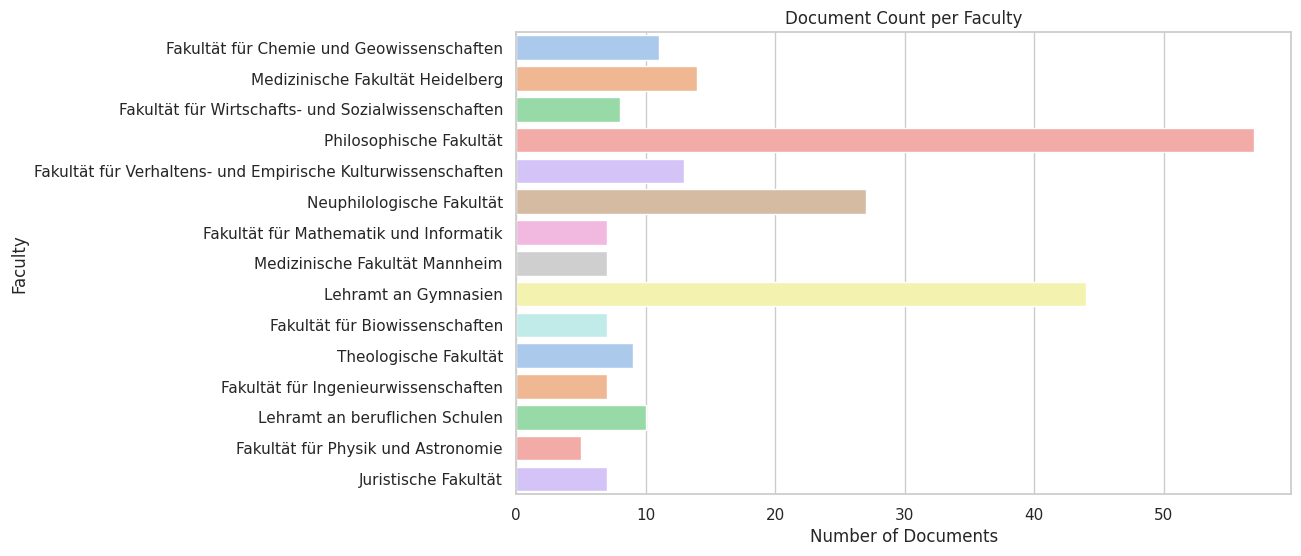
\includegraphics[width=\textwidth]{Grafiken/Statistiken/PO_german_Document Count per Faculty.png}
    \caption{Documents per Faculty of the German \gls{er} Dataset}
    \label{fig:er-german-stats}
\end{figure}

\begin{figure}
    \centering
    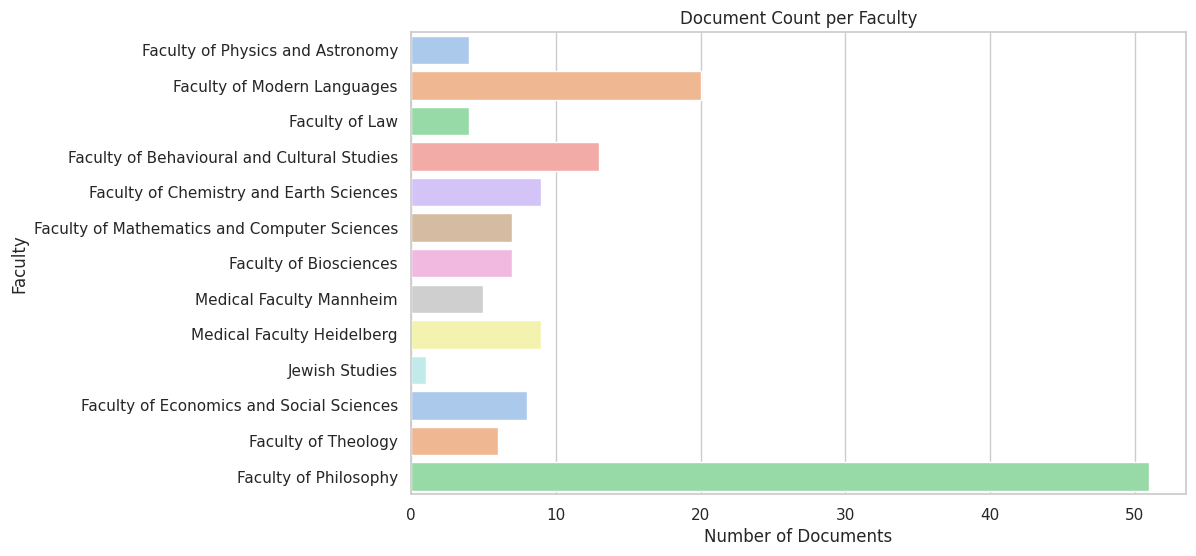
\includegraphics[width=\textwidth]{Grafiken/Statistiken/PO_english_Document Count per Faculty.png}
    \caption{Documents per Faculty of the English \gls{er} Dataset}
    \label{fig:er-english-stats}
\end{figure}

While the previous statistics described the underlying documents of the \gls{poc}, what's even more interesting are the statistics related to the final knowledge source of passages that will be used throughout the \gls{poc}. Details on how these passages have been extracted from the PDFs will be provided in Section \ref{subsec:index}. In this section, we will focus on the statistical analysis.

\begin{figure}
    \centering
    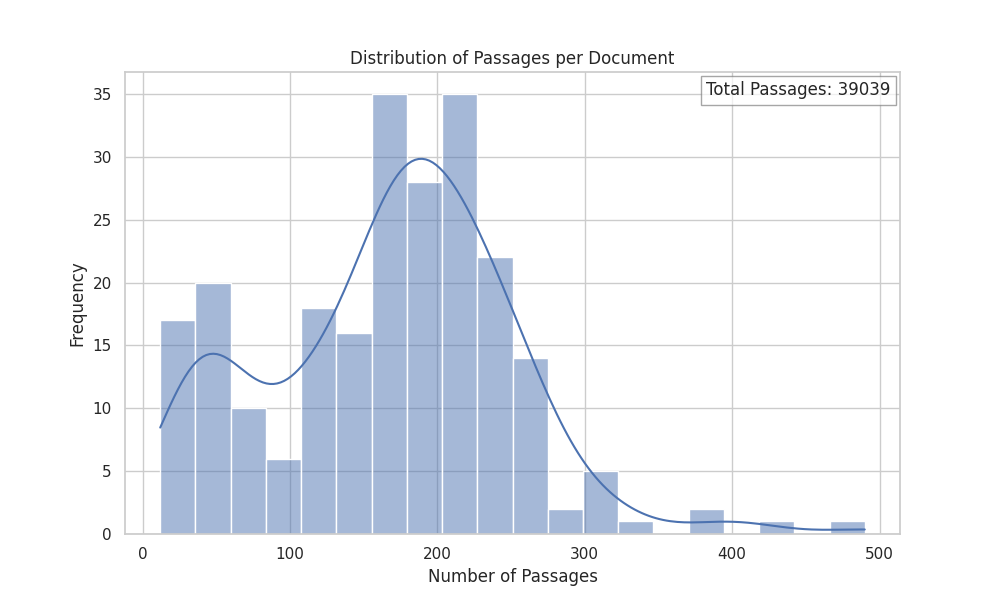
\includegraphics[width=\textwidth]{Grafiken/Statistiken/IndexGerman_Passages_Distribution.png}
    \caption{Passages per Document of the German \gls{er} Dataset}
    \label{fig:er-german-passage-document}
\end{figure}

\begin{figure}
    \centering
    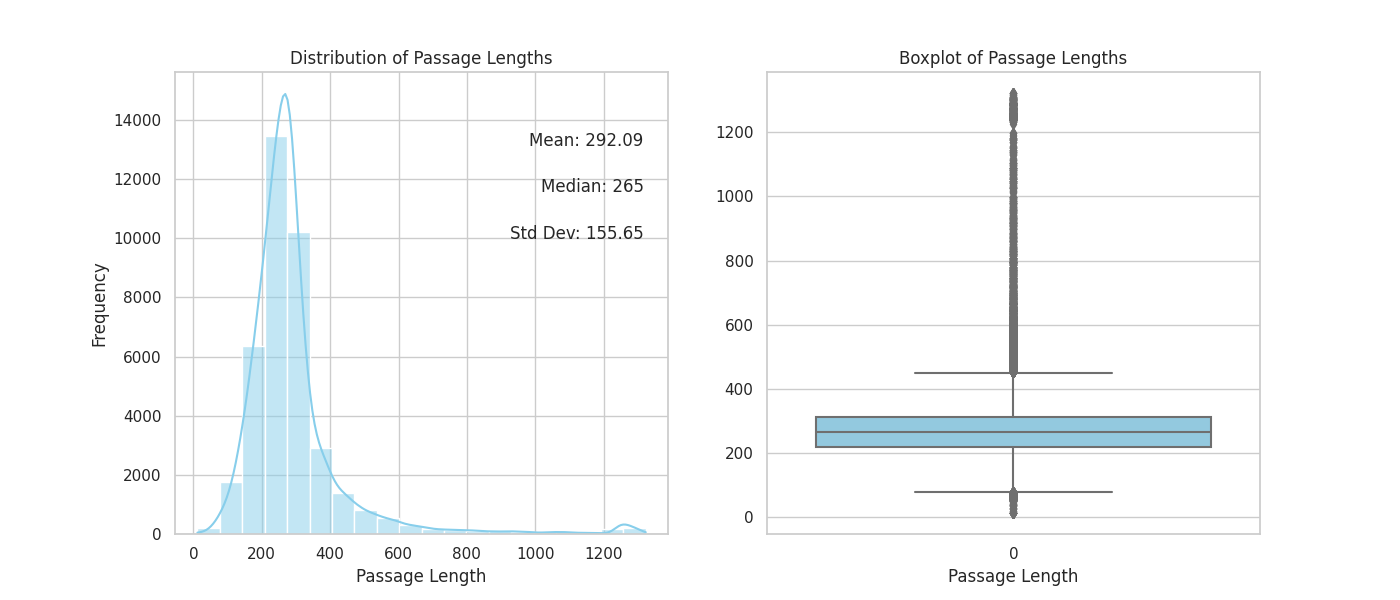
\includegraphics[width=\textwidth]{Grafiken/Statistiken/IndexGerman_Passage_Length_Statistics.png}
    \caption{Passage Length Distribution of the German \gls{er} Dataset}
    \label{fig:er-german-passage-length}
\end{figure}
Figure \ref{fig:er-german-passage-document} illustrates the distribution of passages across documents in the German dataset, offering insights into the diverse influence that documents can have on the knowledge source in terms of the number of passages. These differences in passages are mainly due to variations in the length of the examination regulations (\gls{er}). The total number of passages in the German dataset is 39,039, resulting in an average of 167.55 passages per document. In comparison, the English dataset has an average of 212.94 passages per document. The statistics for the translated dataset are similar to those of the German dataset. An apparent difference between these two datasets is that the distribution of German passages per document exhibits a slight camel-like shape with a local maximum, while the English distribution follows a clear Gaussian pattern. However, these distribution differences are not further evaluated, as we assume that they do not significantly impact the system's quality.

Figure \ref{fig:er-english-passage-document} presents the same statistics for the English dataset. As observed, the English knowledge source is smaller (31,659 vs. 38,642) than the German one, which is expected given that the English dataset contains only 151 \gls{er} compared to the 233 German \gls{er}. Still, the average number of passages per document is higher in the English dataset, as mentioned earlier. The total number of passages in the knowledge source indicates a highly closed-domain scenario. For comparison, MS MARCO \cite{bajaj2016ms}, an often-used dataset for open-domain \gls{qa}, has a knowledge source comprising 3.2 million passages, with an average length of 442 characters and passages ranging from 19 to 1,167 characters.

Figure \ref{fig:er-german-passage-length} depicts the distribution of passage lengths in the German dataset. It's evident that the majority of passages fall within the range of 200 to 350 characters. The same statistics for the English dataset are presented in Figure \ref{fig:er-english-passage-length}. As observed, they are quite similar. The shortest passage is 5 characters, as we applied a lower filter to the extracted passages. The longest passages are 1,300 characters long, also subjected to filtering. Considering statistics such as standard deviation, mean, and median, the English and German datasets do not significantly differ in terms of passage length.


\begin{figure}[H]
    \centering
    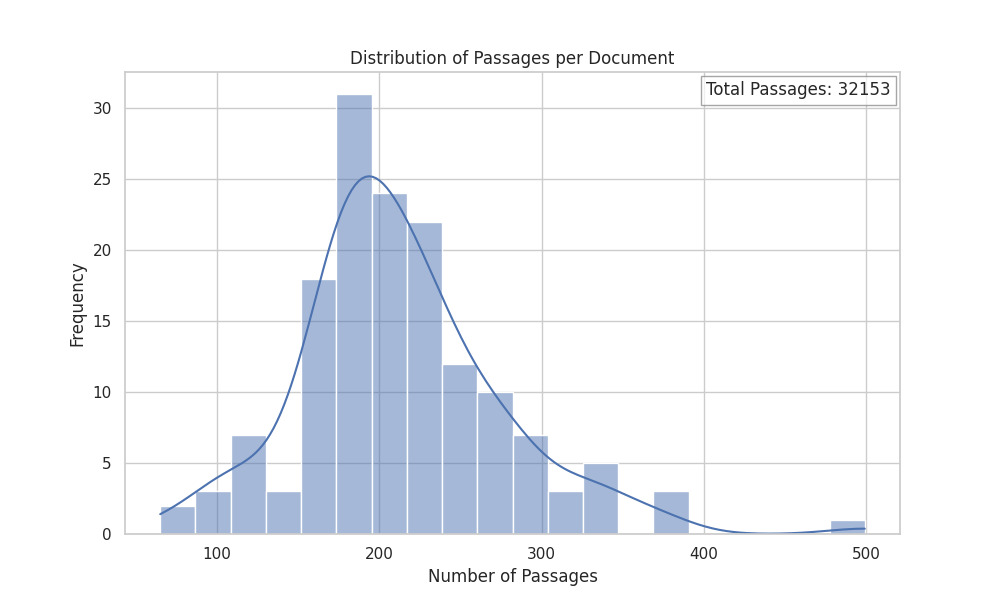
\includegraphics[width=\textwidth]{Grafiken/Statistiken/IndexEnglish_Passages_Distribution.png}
    \caption{Passages per Document of the English \gls{er} Dataset}
    \label{fig:er-english-passage-document}
\end{figure}

\begin{figure}[H]
    \centering
    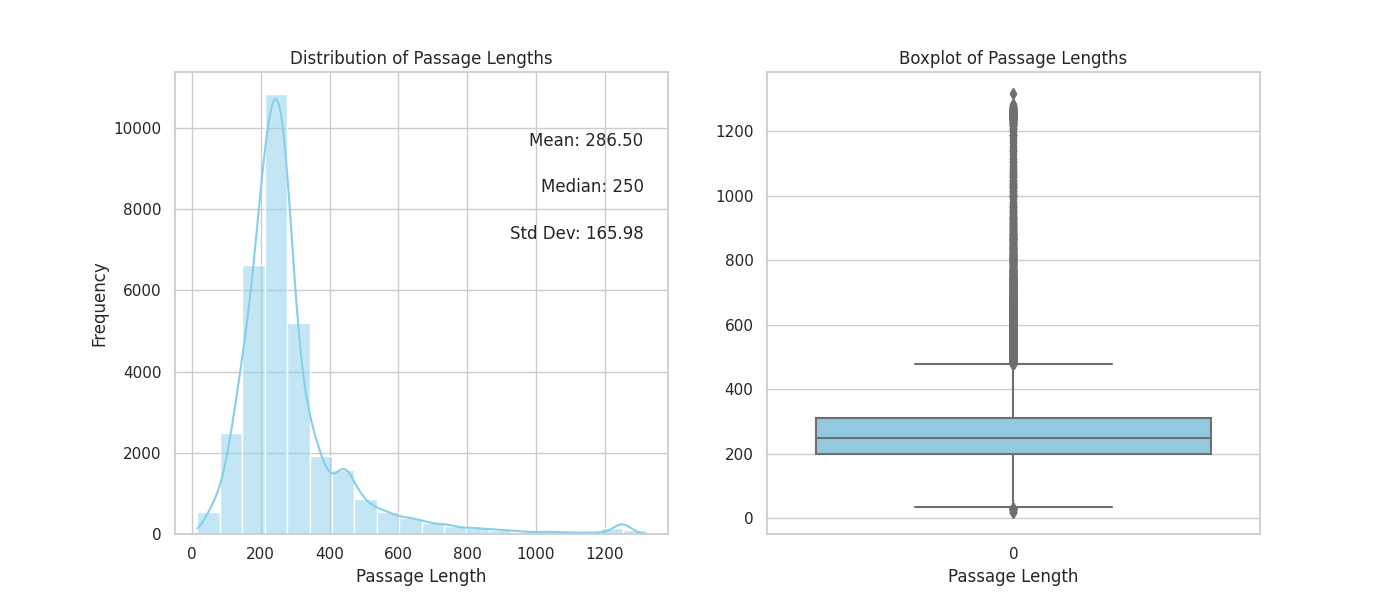
\includegraphics[width=\textwidth]{Grafiken/Statistiken/IndexEnglish_Passage_Length_Statistics.png}
    \caption{Passage Length Distribution of the English \gls{er} Dataset}
    \label{fig:er-english-passage-length}
\end{figure}


\section{Evaluation Approach}
\label{sec:metrics}

The evaluation of a \gls{rag} system, especially in the context of \gls{convqa}, is not trivial. Two known tools/frameworks for this task are RAGAS \cite{noauthor_ragas} and TruLens \cite{noauthor_truelens}. Additionally, the survey by Gao et al. \cite{gao_retrieval-augmented_2024} provides a holistic perspective on the evaluation of \gls{rag} systems. In general, it is useful to evaluate the performance of each individual component (Retriever and Reader) separately in relation to the user's question. The outputs of the Retriever and Reader, namely the Evidence Set and the Answer, can be assessed in different aspects concerning each other and the user's question:

\begin{itemize}
    \item \textbf{Answer Relevance:} How relevant is the Answer in relation to the Question?
    \item \textbf{Context Relevance:} How relevant is the Evidence Set in relation to the Question?
    \item \textbf{Faithfulness:} Are the facts in the Answer based on the facts of the passages in the Evidence Set?
    \item \textbf{Noise Robustness:} How robust is the Reader against noise in the Evidence Set and can it reflect that in the Answer?
    \item \textbf{Negative Rejection:} How well can the Reader determine if the Evidence Set does not contain the answer to the Question and reflect that in the Answer?
\end{itemize}

Figure \ref{fig:evaluation-dimensions} displays the composition of the specific entities and evaluation aspects.

\begin{figure}[H]
    \centering
    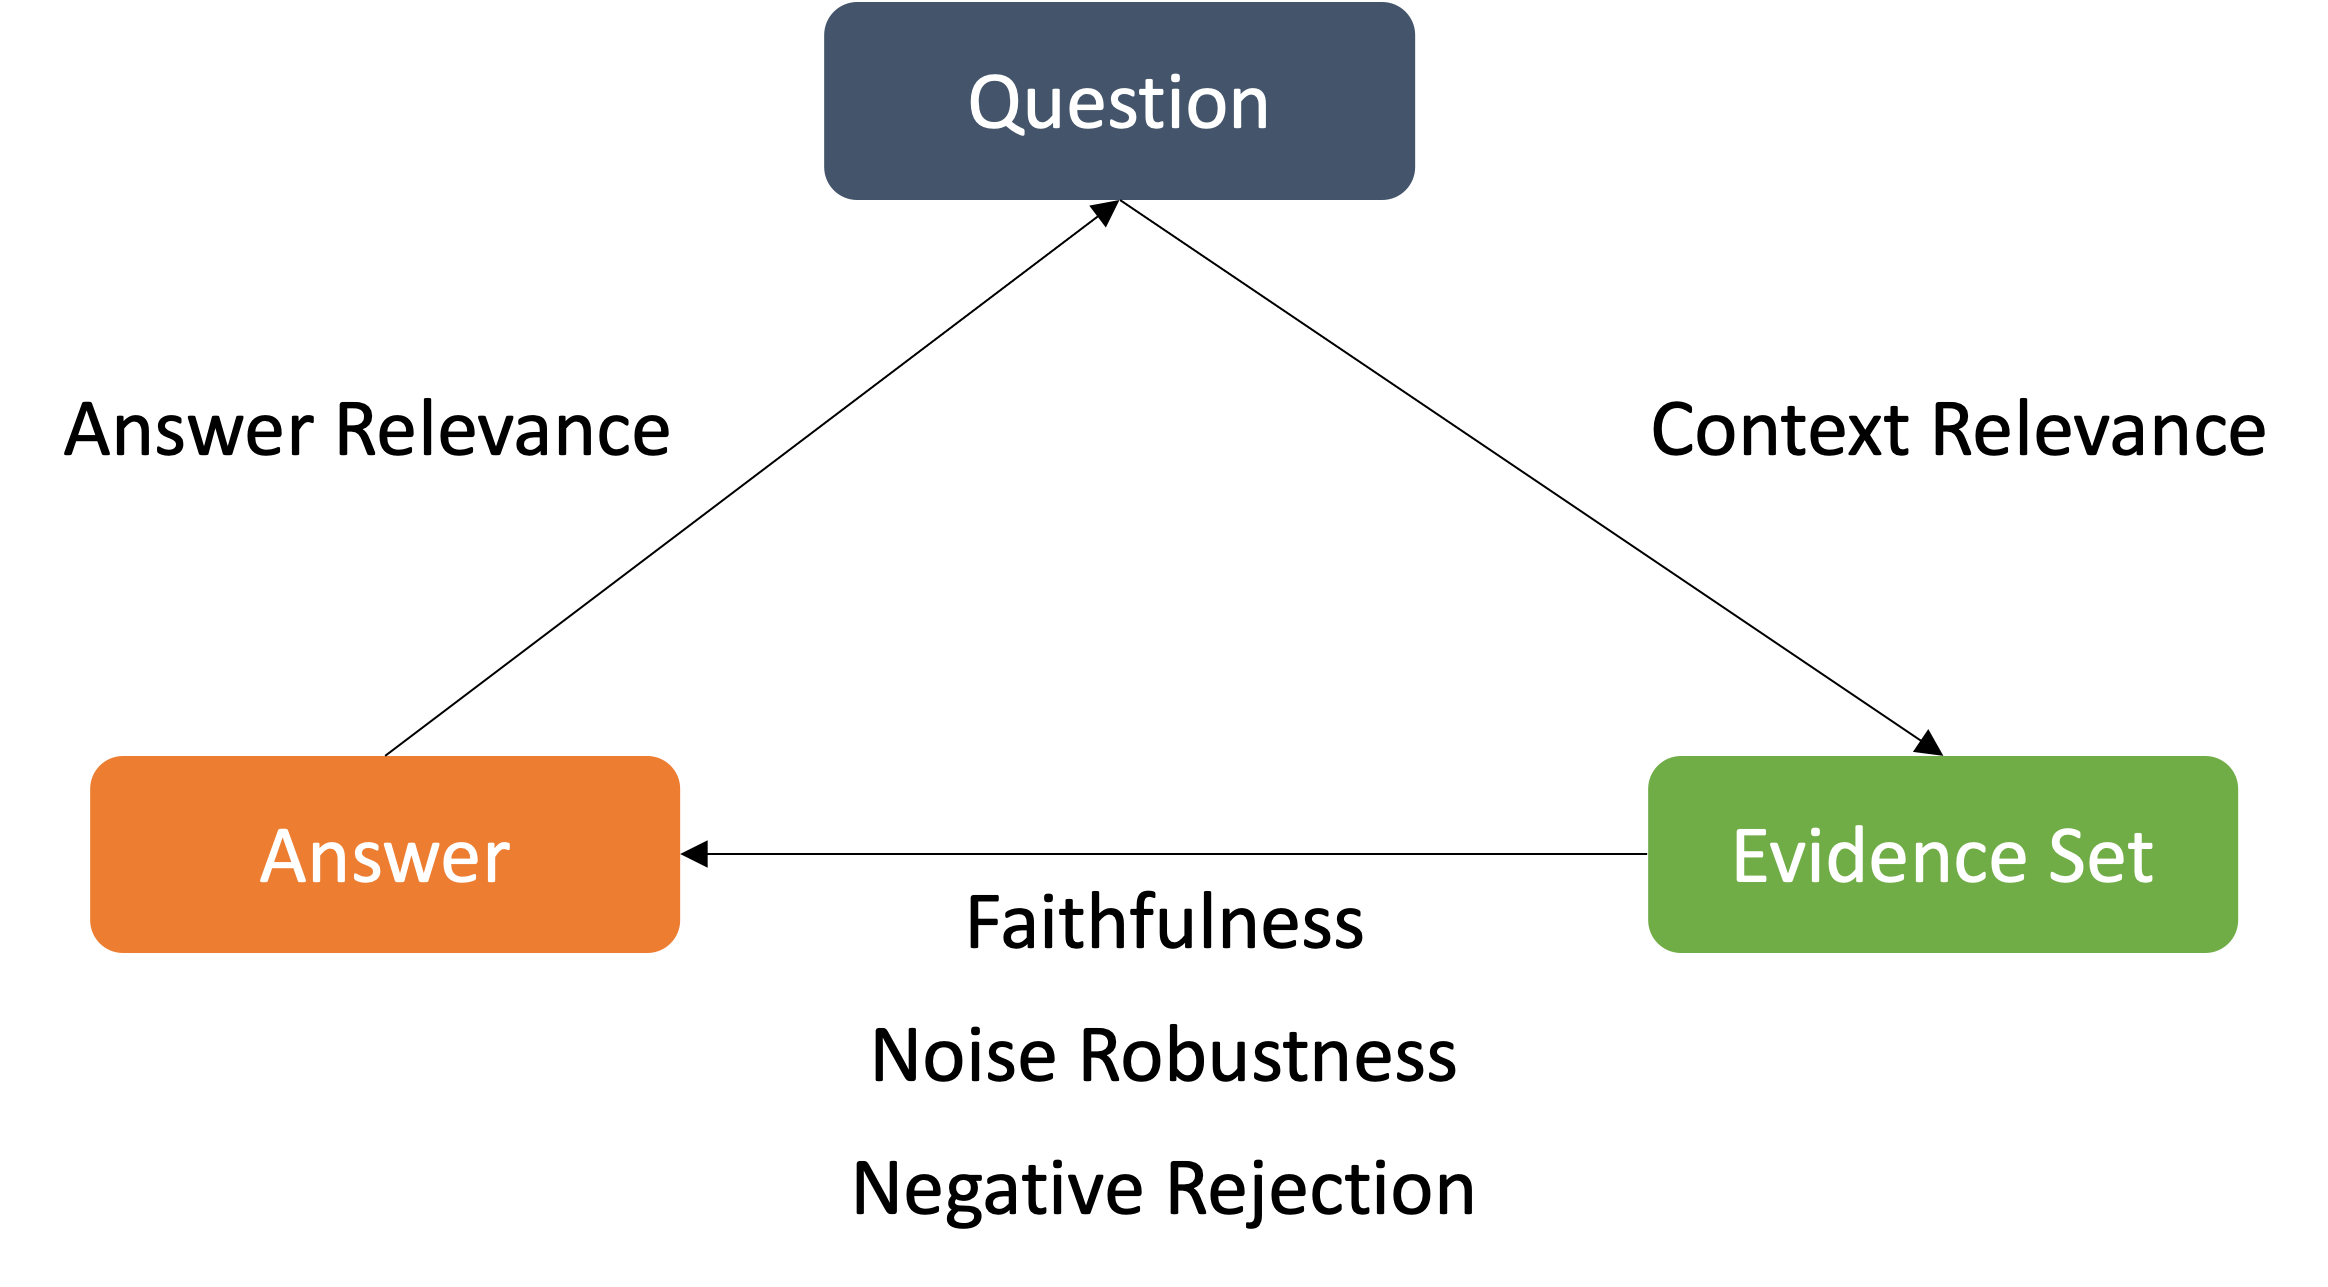
\includegraphics[width=0.8\textwidth]{Grafiken/Evaluation_Dimensions_RAGAS_Turelens.png}
    \caption{Adapted Evaluation Aspects and Components by TruLens \cite{noauthor_truelens}}
    \label{fig:evaluation-dimensions}
\end{figure}

Both the Reader and Retriever components will be evaluated offline using a synthetic dataset. This allows for the identification of the aforementioned aspects for the components in an isolated setting with only one turn, thus in a non-conversational setting. Section \ref{subsec:retrieval-eval} discusses metrics used for the Retriever evaluation, while Section \ref{subsec:answer-generation-eval} introduces metrics for the Reader evaluation.

To evaluate the overall end-to-end performance of the final Conversational Retrieval-Augmented Generation (\gls{conrag}) system, an online approach will be taken. This means that real conversations will be collected, and based on these collected data, evaluation will be conducted. Other approaches may include the generation of synthetic conversations, but this approach will not be covered in this thesis as it cannot be guaranteed with the used smaller \gls{llm}s to create high-quality conversational data. Additionally, to the best of our knowledge, there currently exists no state-of-the-art method for conversation generation based on a knowledge base. Section \ref{subsec:rag-eval} elaborates on this end-to-end approach and the used metrics.

% When it comes to evaluation metrics, it's important to differentiate between the components or models being evaluated. For the evaluation, we will categorize the evaluation scopes as follows:

% \begin{enumerate}
%     \item Retrieval
%     \item Reader
%     \item Conversational Question Answering
% \end{enumerate}

% Evaluating the \gls{cqu} component is only possible with high quality human supervised datasets, therefore for the performance of the \gls{cqu} Section \ref{subsec:cqu-impl} refers to previously by other works performed benchmarks of the used zero-shot models. The exact metrics and paradigms for each individual evaluation will be discussed in the following sections.

\subsection{Retrieval Evaluation Metrics}
\label{subsec:retrieval-eval}

Evaluating a Retriever largely depends on the use-case and the evaluation data available. Since the data introduced in Section \ref{sec:data} lacks a supervised dataset for $(question,\allowbreak passages)$ pairs, we will evaluate it using the synthetic dataset created, as also established in Section \ref{sec:data}. This dataset consists of $(question, passages)$ pairs, where for every question, there is an exact matching passage. Therefore, this dataset is essentially a binary task, where a passage is either the correct one or not. An alternative approach would be a graded relevance task, where each passage has a certain relevance score in relation to the question. However, for our use-case, we opted for the simpler metrics \gls{hr}@k and \gls{mrr}, instead of the Normalized Cumulative Gain (NDCG) used in benchmarks like BEIR \cite{thakur_beir_2021}. We chose these metrics because it's crucial for our system to retrieve the correct passage, and we don't have a relevance score for every passage in relation to every question.

Given a pair of $(q,\hat{p})$, where $\hat{p}$ corresponds to the correct passage and $\forall q, \exists ! \hat{p} \in P$ and a retriever model $p_\eta(p|q) = \text{Score}(q,p)$ (as defined in Definition \ref{eq:retriever}) that assigns a score to every passage $p \in P$ in relation to the question $q$ is used. We can rank all passages based on their relevance to $q$. Each passage receives a rank $r_q,p$ based on its score in relation to $q$. These passages are then ranked in descending order of $r_q,p$, and the top $k$ passages are added to the retrieved set $R_q$.

\begin{itemize}
    \item \textbf{\gls{hr}@k} This metric calculates the proportion of questions for which the correct passage is retrieved within the top $k$ retrieved passages.
    \begin{equation}
        \text{HR@k} = \frac{1}{|Q|} \sum_{q \in Q} 
        \begin{cases}
            1 & \text{if } \hat{p}_q \in R_{q,k} \\
            0 & \text{otherwise}
        \end{cases}
        \in [0,1]
    \end{equation}
    The \gls{hr}@k is a straightforward metric that provides a value between 0 and 1, with a higher value indicating the percentage of cases where the correct passage was retrieved within the top $k$ passages.
    \item \textbf{\gls{mrr}} This metric computes the mean reciprocal rank of the correct passage. It is similar to \gls{hr}@k but considers the position of the correct passage $\hat{p}q$ within the ranking $R_q$.
    \begin{equation}
        \text{MRR} = \frac{1}{|Q|} \sum_{q \in Q} \frac{1}{r_{q,\hat{p}_q}} \in [0,1]
    \end{equation}
    In an ideal system, the \gls{mrr} would be 1, indicating that the correct passage is always retrieved in the first position ($r_{q,\hat{p}} = 1$) for all $q \in Q$.
\end{itemize}

\subsection{Reader Evaluation Metrics}
\label{subsec:answer-generation-eval}

Evaluating the task of answer generation, particularly the \gls{mrc} aspect of the reader component, presents challenges similar to those discussed for the retrieval task evaluation in Section \ref{subsec:retrieval-eval}. For automatic and manual evaluation, we will utilize the synthetic dataset generated in Section \ref{sec:data}. This dataset comprises triples of $(\text{question}, \text{passages}, \text{answer})$, where \textit{answer} refers to a gold answer that has been syntactically generated.

In the context of a triple $(q, \hat{p}, \hat{a})$, where $\hat{p}$ corresponds to the correct passage and $\hat{a}$ corresponds to the correct answer in relation to a question $q$, we employ a reader model $r_{\text{k-Reader}}(E_{q_c}, q_c,H) := a_i$ (as defined in Definition \ref{eq:reader}) to predict the answer $\hat{a}$ given the question $q$ and the passage $\hat{p}$. The predicted answer $a'$ is then evaluated using the following metrics:

\begin{itemize}
    \item \textbf{BLUE-1:} This precision-oriented metric compares the occurrence of unigrams (words $w \in \hat{a}$) in the predicted answer $a'$ and the gold answer $\hat{a}$.
    \begin{equation}
        \text{BLUE-1} = \frac{\sum_{w \in a'} \min(\text{count}_{a'}(w), \text{count}_{\hat{a}}(w))}{\sum_{w \in a'} \text{count}_{a'}(w)} \in [0,1]
    \end{equation}
    Here, $\text{count}_{a'}(w)$ represents the number of occurrences of the word $w$ in the predicted answer $a'$. \gls{bleu} is particularly useful for evaluating extractive questions \cite{papineni_bleu_2002}.

    \item \textbf{ROUGE-L:} This recall-oriented metric, especially \gls{rogue}-L, compares the longest common subsequence ($LCS$) between the predicted answer $a'$ and the gold answer $\hat{a}$.
    \begin{align}
        R_{LCS} &= \frac{LCS(\hat{a}, a')}{|\hat{a}|} \\
        P_{LCS} &= \frac{LCS(\hat{a}, a')}{|a'|} \\
        \text{ROUGE-L} &= \frac{(1+\beta^2)R_{LCS}P_{LCS}}{R_{LCS}+\beta^2P_{LCS}} \in [0,1]
    \end{align}
    Here, $\beta$ is a parameter to balance between precision and recall. Rouge operates similarly to \gls{bleu} but focuses on lexical matching \cite{lin_rouge_2004}.

    \item \textbf{F1-BERTscore}: BERTscore is a \gls{s2s}-model-based evaluation metric for comparing two text fragments: $x$, which is the reference, and $\hat{x}$, which is the prediction. In this context, the predicted answer $a'$ is compared to the gold answer $\hat{a}$. Essentially, the score between two tokens, $a'_i$ and $\hat{a}_i$, is calculated as the inner product of their respective BERT embeddings: $\text{BERT}(a'_i)^T\text{BERT}(\hat{a}_i)$. For simplicity, we'll use the  $\text{BERT}(a'_i) \rightarrow a'_i$ in the following equations. The final scores of F1-BERTscore are weighted by the inverse document frequency (idf) of each word-piece token:

    \begin{align}
        P_{BERT} &= \frac{\sum_{a'_j\in a'} \text{idf}(a') \max_{\hat{a}_i \in \hat{a}} (\hat{a}_i^T a'_j)}{\sum_{a'_j\in a'} \text{idf}(a')} \\
        R_{BERT} &= \frac{\sum_{\hat{a}_i \in \hat{a}} \text{idf}(\hat{a}_i) \max_{a'_j \in a'} (\hat{a}_i^T a'_j)}{\sum_{\hat{a}_i \in \hat{a}} \text{idf}(\hat{a}_i)} \\
        F1_{BERT} &= \frac{2P_{BERT}R_{BERT}}{P_{BERT}+R_{BERT}}
    \end{align}
    
    The advantage of F1-BERTscore lies in its reliance on semantic matching between the gold answer $\hat{a}$ and the predicted answer $a'$ rather than mere lexical matching \cite{zhang_bertscore_2020}.
    

    \item \textbf{Accuracy} This metric calculates the proportion of questions for which the predicted answer $a'$ matches the gold answer $\hat{a}$. 
    \begin{equation}
        \text{Accuracy} = \frac{1}{|Q|} \sum_{q \in Q} 
        \begin{cases}
            1 & \text{if } a' = \hat{a} \\
            0 & \text{otherwise}
        \end{cases}
        \in [0,1]
    \end{equation}
    This metric is useful for evaluating question, answer realtions, where there is only one correct answer. In order to define if an answer is correct or not, the following approaches will be used:
    \begin{itemize}
        \item \textbf{LLM-based:} A \gls{llm} can be prompted to determine a binary value (0 or 1) indicating whether the underlying message of $a'$ and $\hat{a}$ matches. The prompt used is based on the work of \cite{kamalloo_evaluating_2023}:
        \begin{quote}
            \texttt{Question:} q \\
            \texttt{Gold Answer:} $\hat{a}$ \\
            \texttt{Predicted Answer:} a' \\
            \texttt{Is the predicted answer correct?} Yes/No
        \end{quote}
        This approach is especially useful for evaluating generative questions, as it allows for semantic matching.
        \item \textbf{Human-based:} In this approach, a human evaluator is asked to assign a binary value of 0 or 1, indicating whether there is a match in the underlying message of $a'$ and $\hat{a}$. The evaluator assigns 1 if the answer $a'$ covers the information from $\hat{a}$ and 0 if it does not. The evaluator is provided with the question $q$, the important passage $\hat{p}$, the gold answer $\hat{a}$, and the generated answer $a'$. This approach is particularly useful for evaluating generative questions and closely resembles real-world applications. In addition to indicating accuracy, the evaluator gives a binary value of 0 or 1 to indicate whether the generated gold answer is correct and another binary value, if the question is an \textit{extractive} question, which is answerable given the context. For this thesis, two evaluators will assess 50 randomly sampled datapoints with the context present in the evidence set and another 50 where the context was dropped. They will assign a binary value to each answer. The inter-rater agreement will be calculated using Cohen's Kappa \cite{cohen_coefficient_1960}.
    \end{itemize}
\end{itemize}

\subsection{End-to-End RAG Evaluation}
\label{subsec:rag-eval}

The most challenging aspect of evaluation within the context of the system developed here is assessing \gls{conrag} as a holistic system. To conduct the evaluation, a dataset of conversations needs to be generated. This will be achieved through interactions of human evaluators engaging in conversations with the system. No automatic metrics will be utilized. Instead, all evaluation aspects will be assessed by human evaluators. There exist evaluation approaches using \gls{llm}s or the embeddings of \gls{dpr} in order to automatically evaluate certain aspects, but those won't be utilized for this limited evaluation dataset. The evaluation process involves the following steps:

\begin{enumerate}
    \item A human evaluator initiates a conversation with a question, either based on their own intuition or using provided questions from the synthetic dataset. Evaluators are encouraged to pose context-dependent questions, which can be answered given a specific passage of the POs or not at all. Complex multi passage questions should be avoided, as this complicates the evaluation process.
    \item The evaluator continues the conversation, asking follow-up questions or engaging in a general discussion with the \gls{convqa}-System for 8-10 turns.
    \item After the conversation, the evaluator has access to the evidence set $E_{q_c}$ for each turn and all other passages $P$ in the index. The evaluator assesses the answer provided by the system and the retrieved evidence set $E_{q_c}$. They are required to provide the following information for every turn of the conversation:
        \begin{itemize}
            \item \textit{Context Relevance:} The evaluator assigns a binary accuracy value (0 or 1), indicating if the evidence set contains the required information to answer the question. A score of 1 indicates that the evidence set contains the required information, while 0 indicates that the evidence set does not contain the required information.
            \item \textit{Noise Robustness:} To have insights on the noise robustness, the evaluator has to indicate via number the position in the evidence set $E_{q_c}$ of the relevant passage. For example, 0 indicates that the first passage in the evidence set is the relevant passage, and 4 indicates that the fifth passage in the evidence set is the relevant passage.
            \item \textit{Faithfulness:} The evaluator assigns a binary value (0 or 1), indicating whether the answer is based on the facts of the evidence set. A score of 1 indicates that the answer is based on the facts of the evidence set, while 0 indicates that the answer is not based on the facts of the evidence set. When the provided evidence set does not indicate any answer and the system provides an answer indicating that it does not have any information on the topic, the evaluator has to assign a score of 1.
            \item \textit{Negative Rejection:} This can be evaluated indirectly via the combination of Context Relevance, Faithfulness, and Answer Relevance.
            \item \textit{Answer Relevance:} The evaluator assigns a value between 0 and 1 to the system's answer. A score of 1 indicates a correct answer to the given question in relation to the conversation history, while 0 represents an incorrect answer.
            \item \textit{Reason for Incorrectness:} The evaluator selects one of the following reasons for incorrectness, only if the answer relevance is 0 and Context Relevance 1: \textit{No Negative Rejection}, \textit{Nonsense Answer}, \textit{Hallucination}, \textit{Coreference Problem}, \textit{Other} (here the evaluator has to provide a short description of the reason for incorrectness) 
        \end{itemize}
    \item All results will be grouped by turn, enabling deeper insights into the performance and errors of the system.
\end{enumerate}

To mitigate bias, human manual evaluations are carried out by two different evaluators. In the first round, each evaluator engages in 10 conversations with the system. In the second round, the evaluators initiate conversations using the first question from the 10 conversations of the other evaluator. This results in a total of 40 conversations, with ideally 20 overlapping conversations that can be used to calculate inter-rater agreement \cite{cohen_coefficient_1960}.
    
% \subsection{Conversational Question Answering Evaluation}
% \label{subsec:convqa-eval}
% The first approach, known as \textbf{\gls{mahueval}}, operates as follows:

% The second approach, \textbf{\gls{auev}}, operates as follows. In this approach, a synthetic dataset is provided, consisting of lists of triples $(q, \hat{p}, \hat{a})$, where each triple corresponds to one turn, and a list represents a conversation history $h \in H$:

% \begin{enumerate}
%     \item Initially, the system is presented with the first question $q_1$ from the conversation history. The response $a'_1$ is evaluated using the \textit{F1-BERTscore} in comparison to the gold answer $\hat{a}$ of the history $h$. This score is computed for each turn, assessing the system's response against the gold answer for that turn.
%     \item Subsequently, to mitigate the impact of an incorrect system response on the ongoing conversation, the following question (e.g., $q_2$) is augmented with the gold answer $\hat{a}_1$. This augmentation helps address missing information or coreference problems caused by an erroneous response. This method, originally introduced by Li et al. \cite{li_ditch_2022}, improves the automatic evaluation of \gls{convqa} systems. The model used to resolve the relationship between the gold answer and the question is the standard CQU model. Additionally, within the \gls{convqa} history, the answer $a'_1$ is replaced by the gold answer $\hat{a}_1$ for the CQU unit.
%     \item After enhancing the question, the system is tasked with generating a response $a'_2$ to the augmented question $q'_2$. Once again, the response $a'_2$ is evaluated using the \textit{F1-BERTscore} against the gold answer $\hat{a}_2$ from the history $h$.
%     \item Steps (2) and (3) are repeated until the end of the conversation history $h$.
%     \item All scores will be groupable by turn depth, enabling deeper insights into the performance and errors of the system.
% \end{enumerate}

% Both \gls{mahueval} and \gls{auev} will be employed to evaluate the \gls{convqa} system, and the results will be reported separately.

\section{Experimental Setup and Implementation}
\label{sec:setup}

This section outlines the experimental setup and provides details on the implementation of the System Architecture and Framework introduced in Chapter \ref{chap:main}. First and foremost, we apply the theoretically outlined model ($M$) to create an implementation decision map. Figure \ref{fig:extract-pipeline-implementation-grid} illustrates a decision tree showcasing the possible implementations of the \textit{Extract} pipeline. Figure \ref{fig:all-components-conrag-grid} displays the main components, namely the \textit{Retriever}, \textit{Reader}, and \textit{\gls{cqu}}, in a similar decision matrix, where each column represents a decision to be made during implementation. Opting not to make a decision is also a valid choice. Developing an implementation can then be easily achieved using a decision tree, as shown in Figure \ref{fig:example-implementation-tree}. For the implementation and benchmarking, ressources of the BwUniCluster\footnote{\url{https://wiki.bwhpc.de/e/BwUniCluster2.0}} have been used. For further details on the model parameters used for all tasks, please refer to the Appendix \ref{ref:appendixA-evaluation-model-configurations}.

\begin{figure}
    \centering
    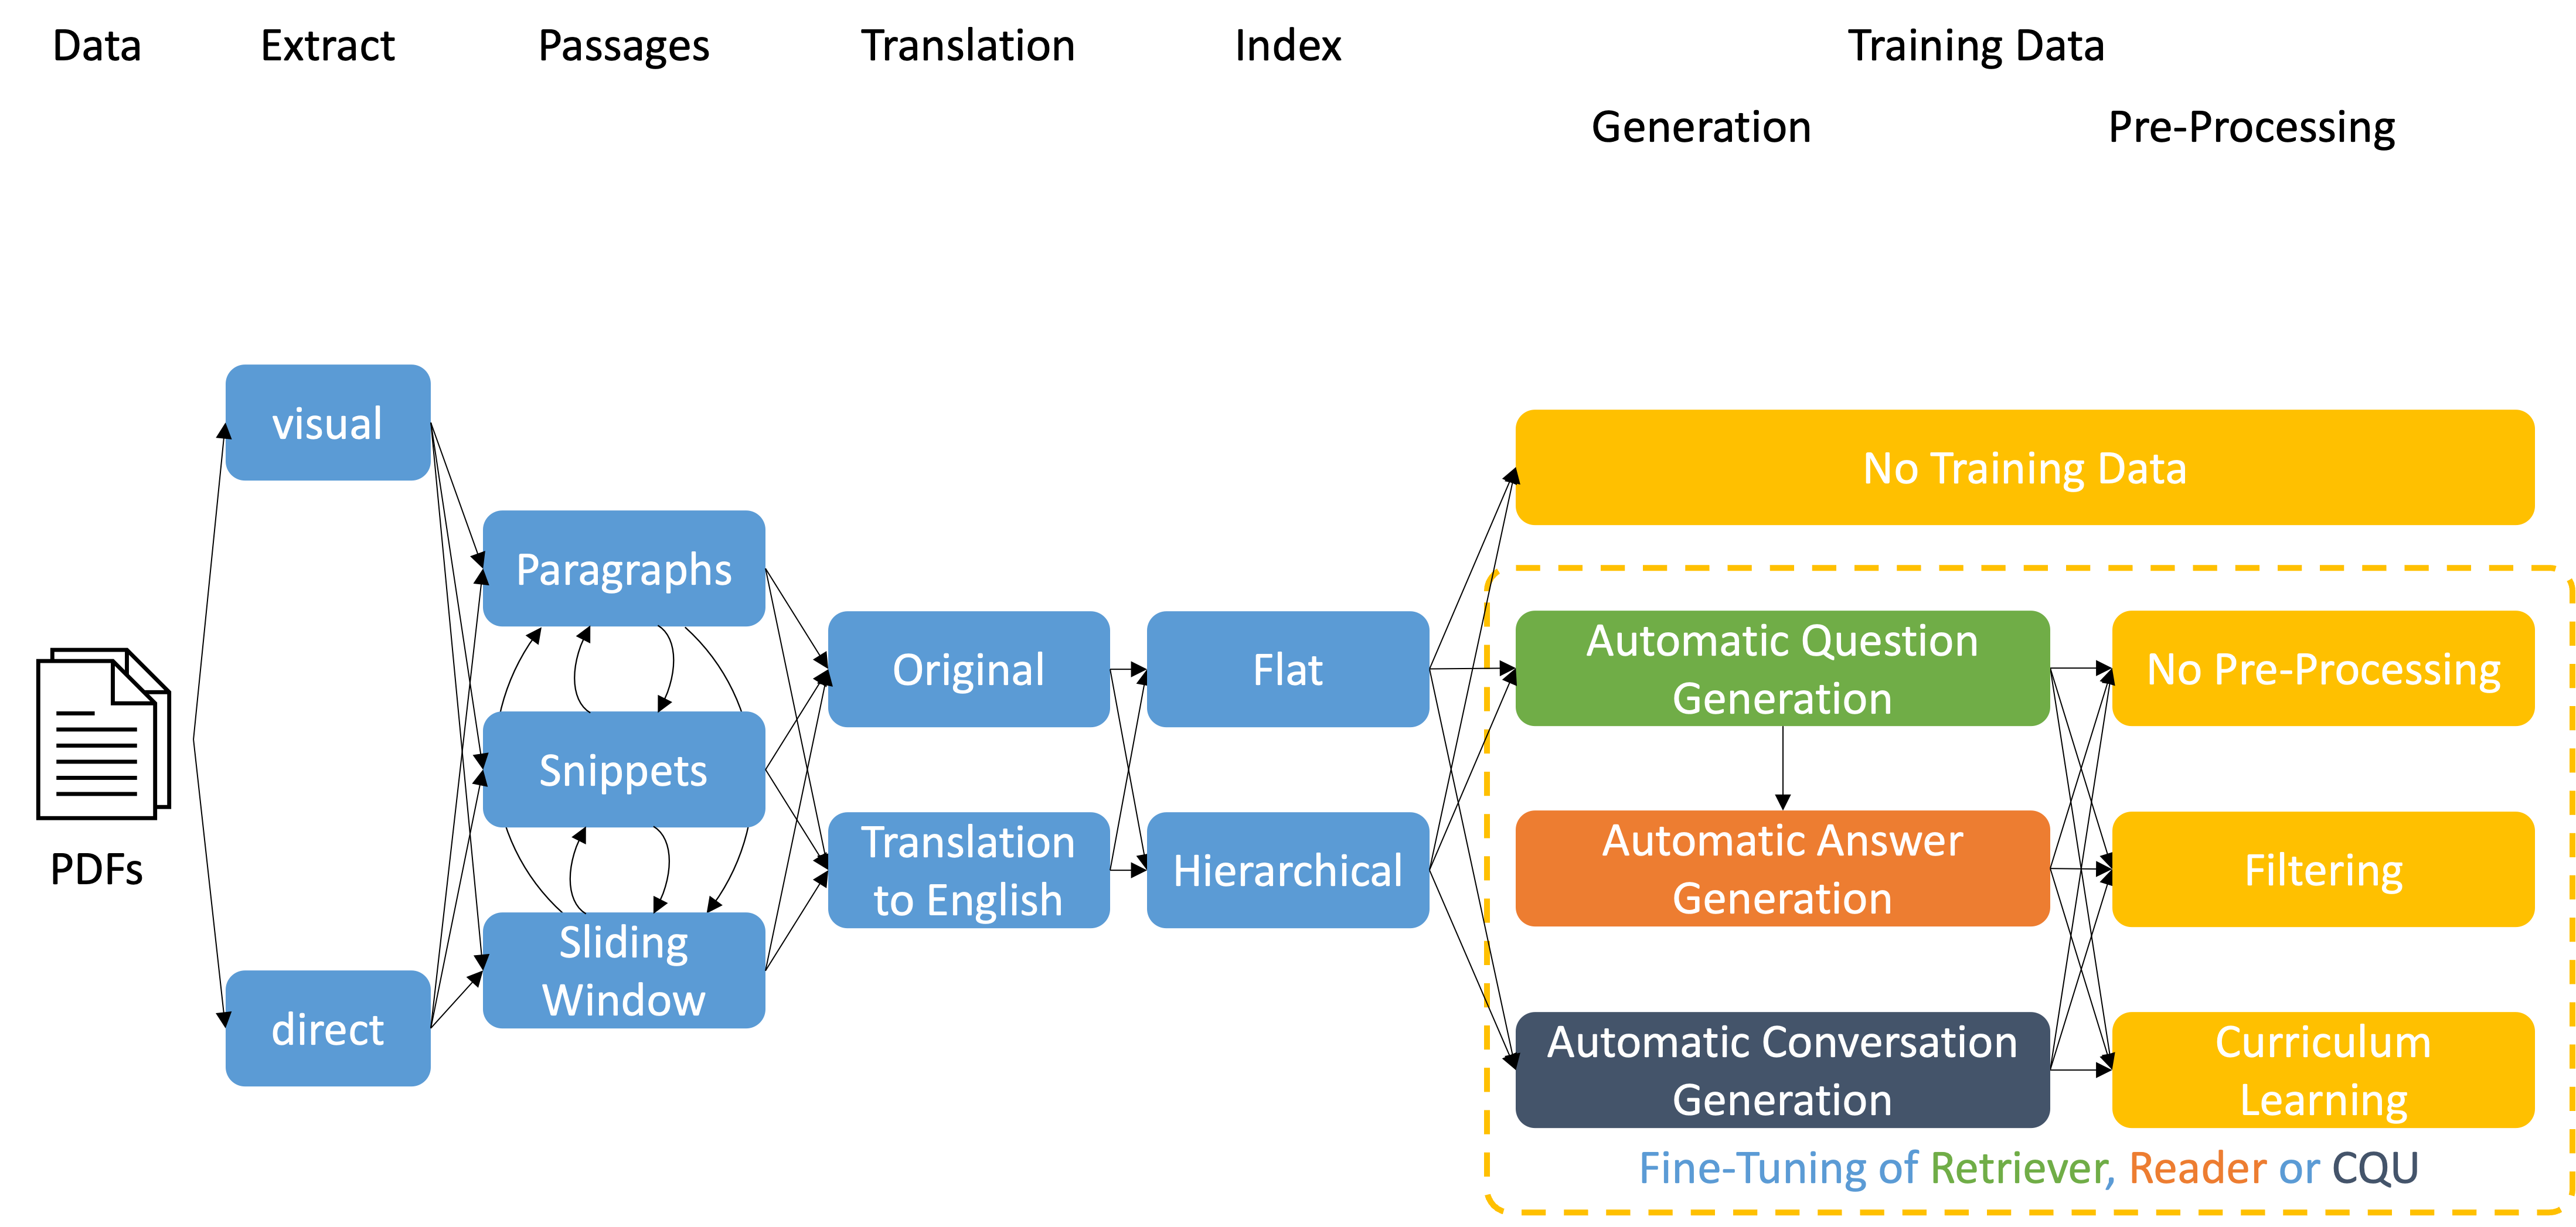
\includegraphics[width=\textwidth]{Grafiken/extract_pipeline.png}
    \caption{Possible Implementations of the Extract Pipeline}
    \label{fig:extract-pipeline-implementation-grid}
\end{figure}

\begin{figure}
    \centering
    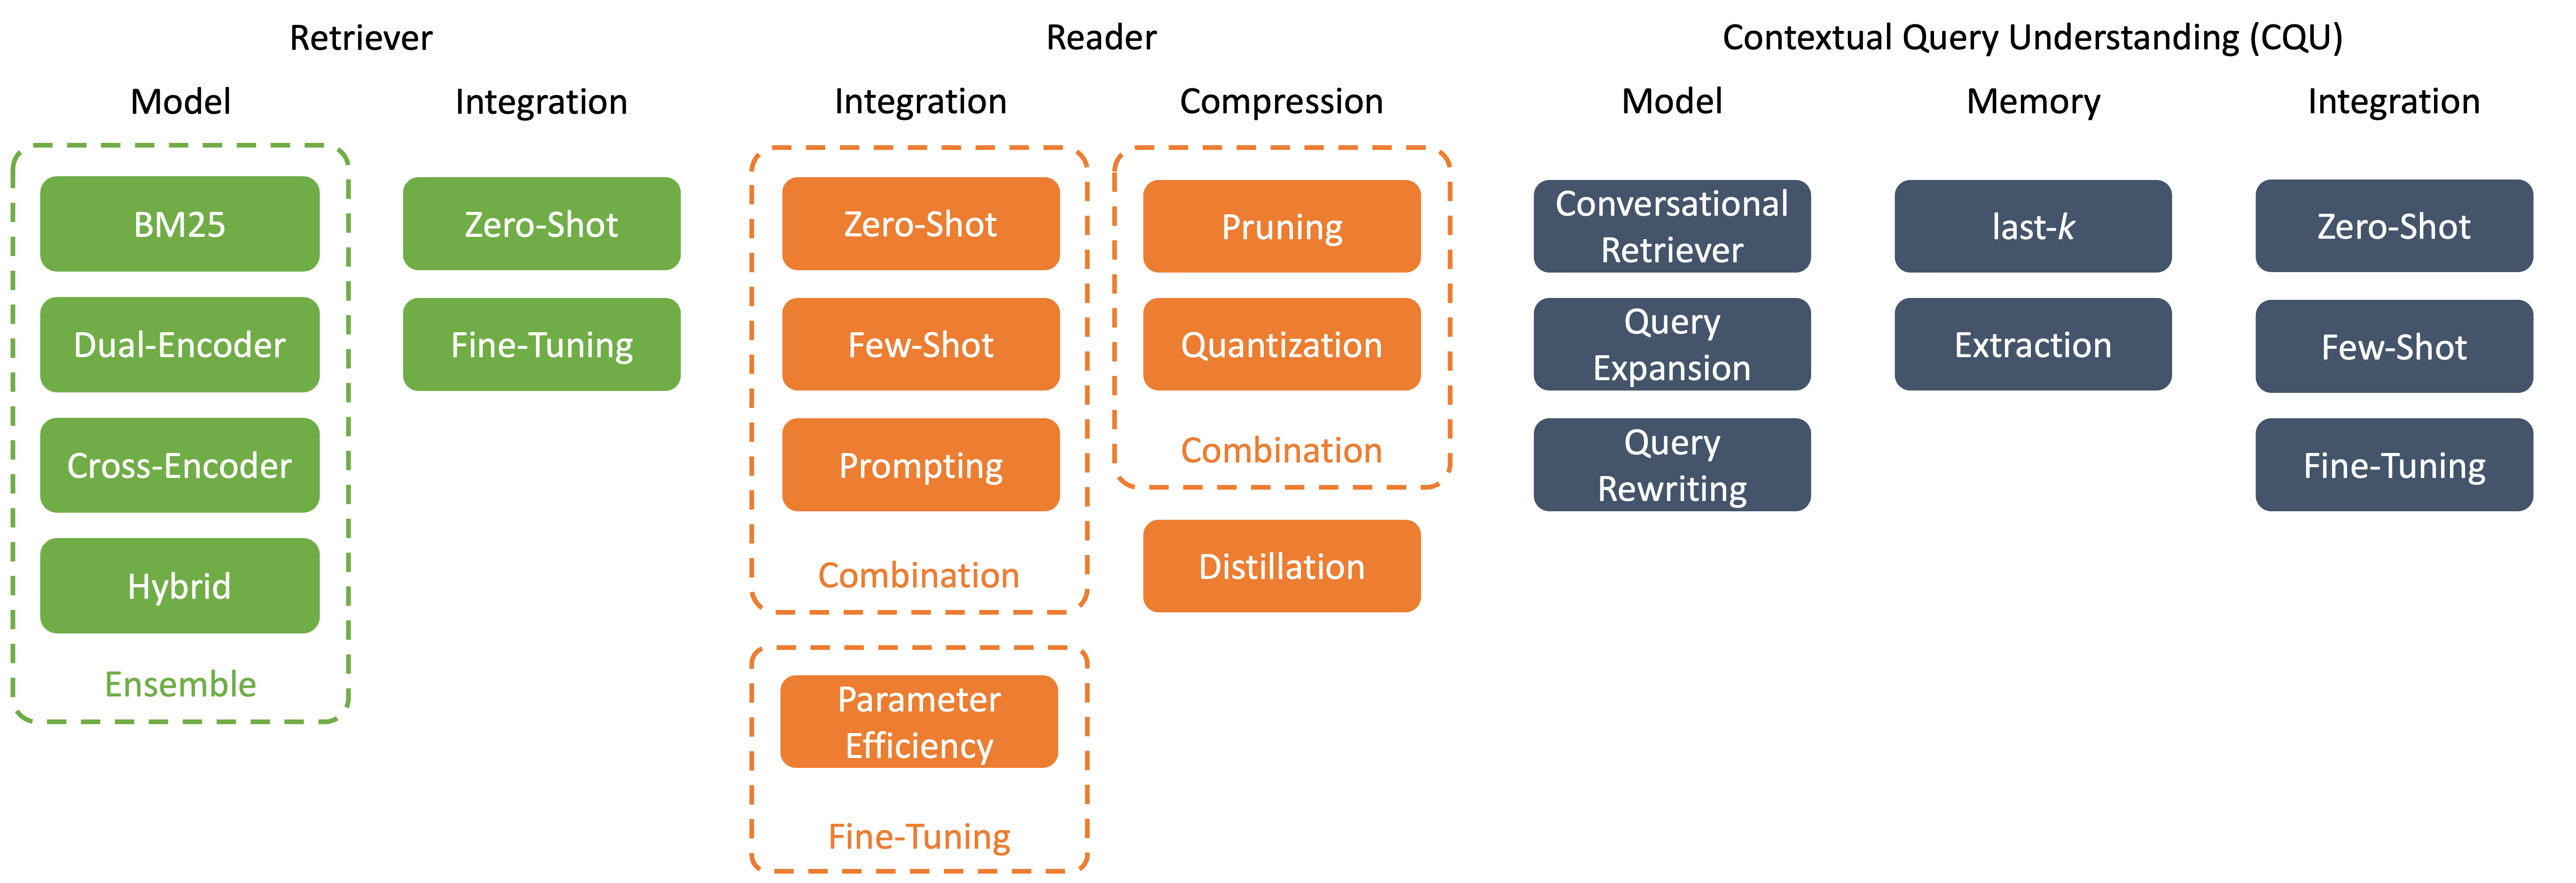
\includegraphics[width=\textwidth]{Grafiken/all_components_conrag.png}
    \caption{All Components of the System Architecture}
    \label{fig:all-components-conrag-grid}
\end{figure}

\subsection{Extraction}
\label{subsec:index}

Figure \ref{fig:extract-pipeline-implementation} illustrates the extraction pipeline implemented for this thesis' \gls{poc}, resulting in the creation of the \textit{document model} of the passages forming the knowledge source. This pipeline comprises the following steps:

\begin{figure}
    \centering
    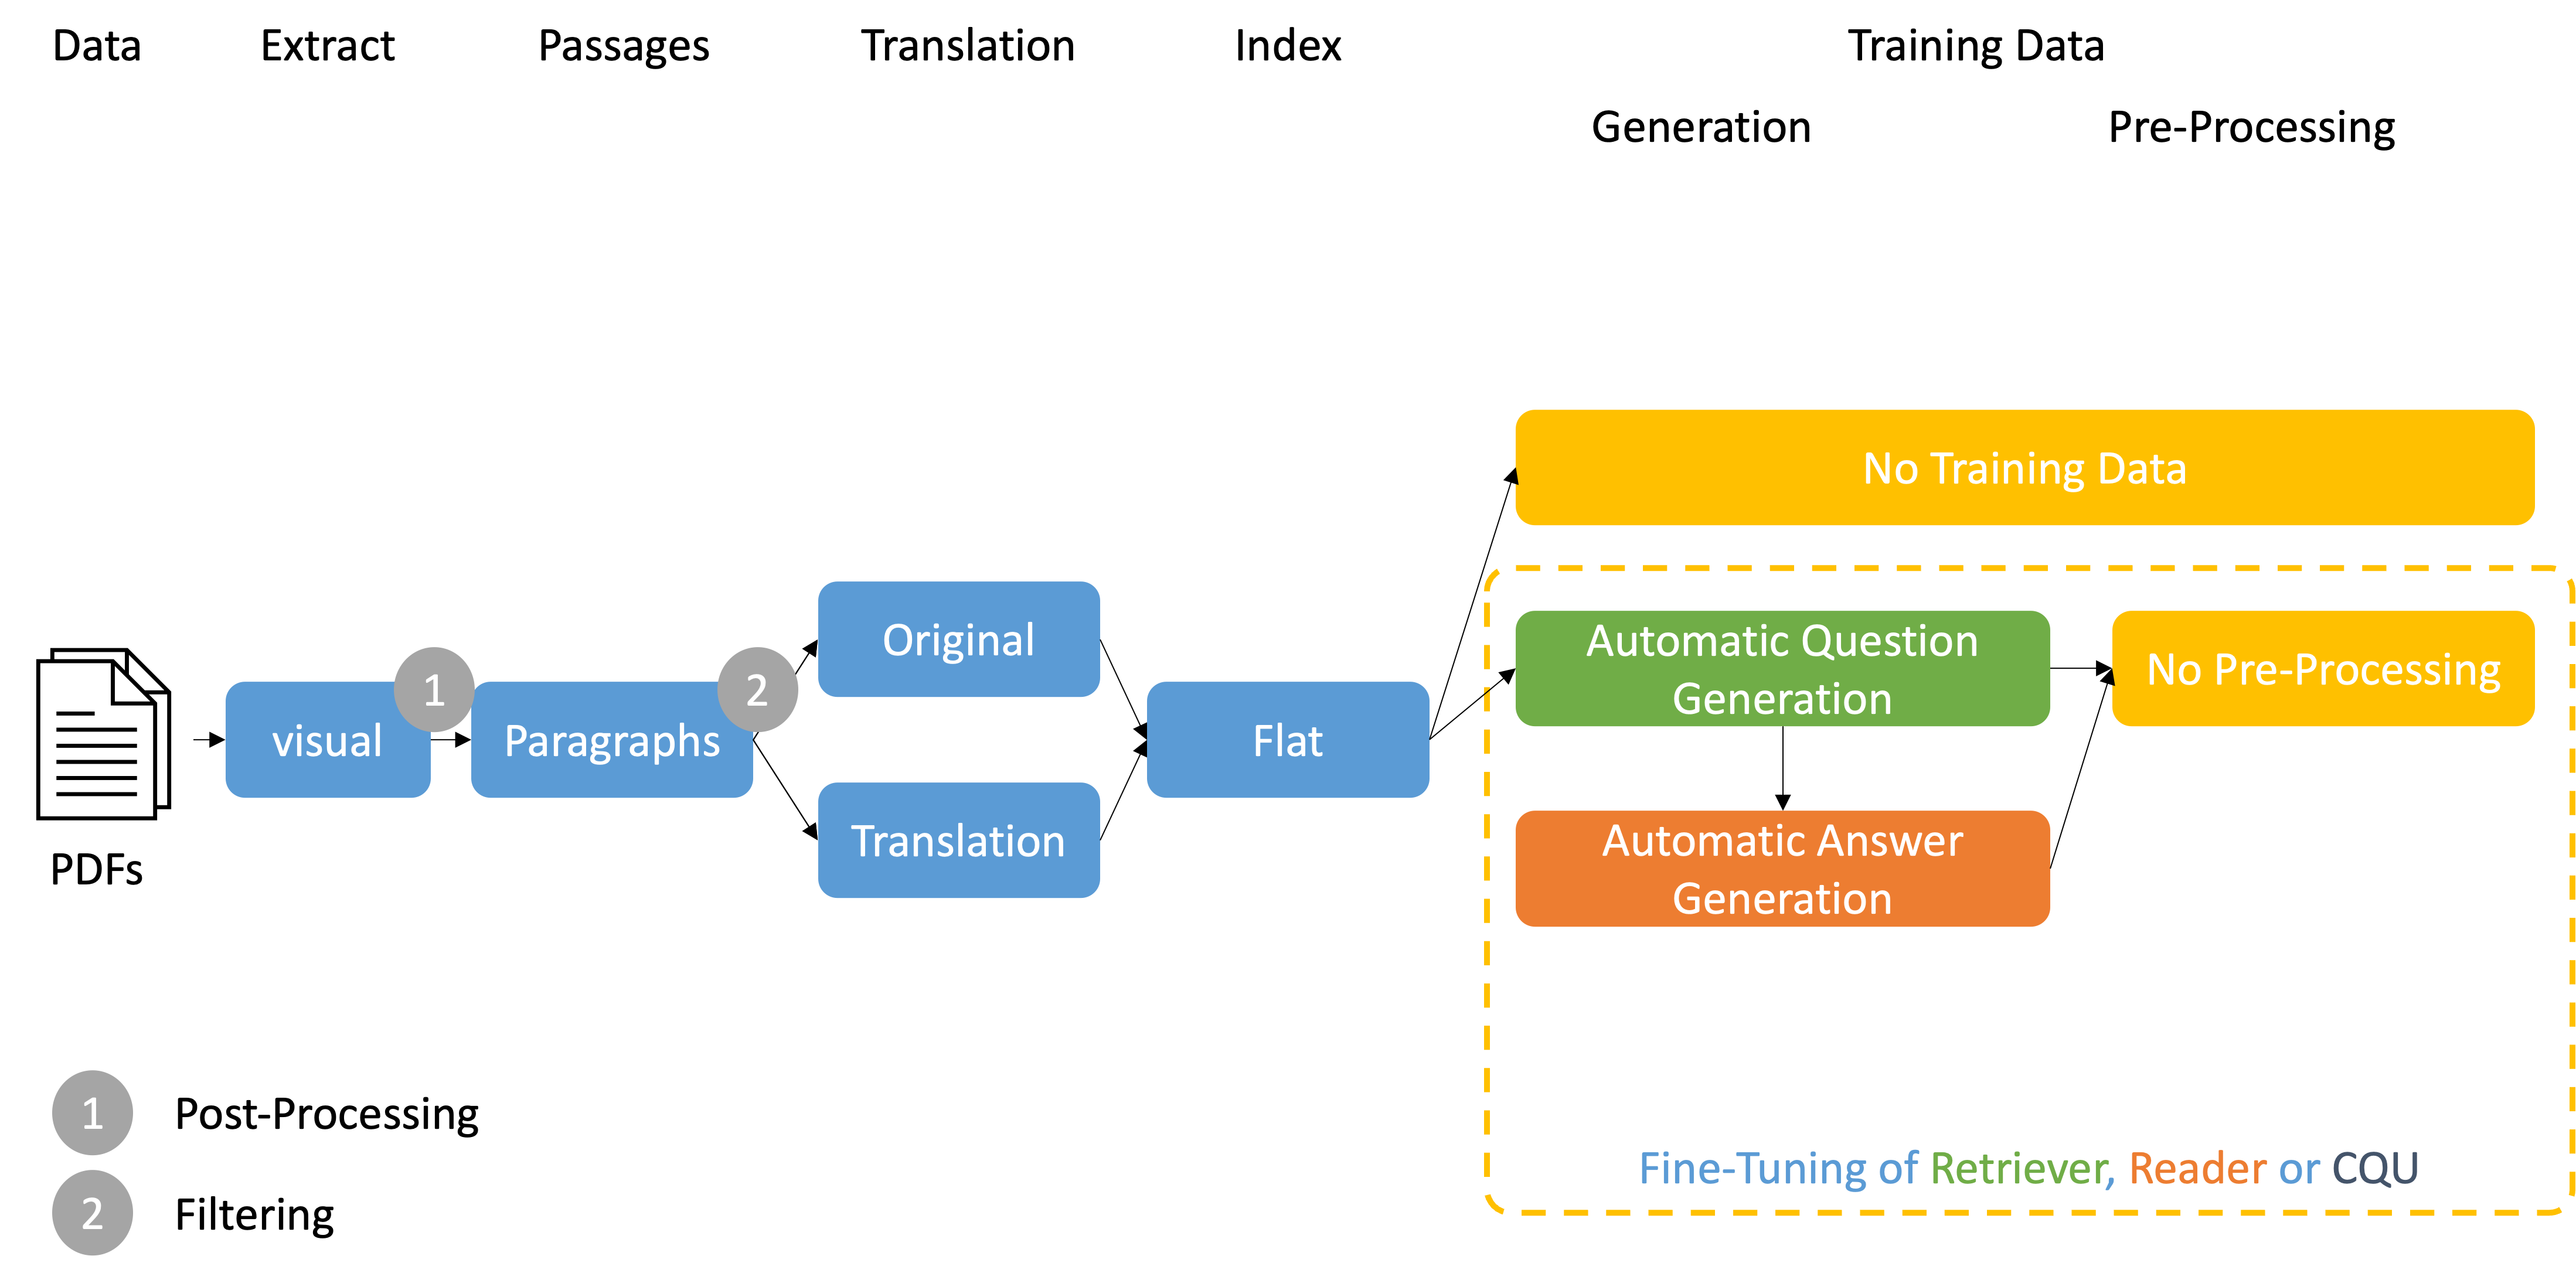
\includegraphics[width=\textwidth]{Grafiken/Evaluation/extract_implemented.png}
    \caption{Implemented Extraction Pipeline}
    \label{fig:extract-pipeline-implementation}
\end{figure}

\begin{enumerate}
    \item \textit{Extract:} Visual extraction using the Google Cloud Vision API for PDF OCR\footnote{\url{https://cloud.google.com/vision/docs/pdf}}, followed by post-processing.
    \item \textit{Passages:} Extraction of paragraphs using the NLTK tokenizer-based Text Splitter by Langchain\footnote{\url{https://python.langchain.com/docs/modules/data\_connection/document\_transformers/text\_splitters/split\_by\_token\#nltk}}, followed by filtering.
    \item \textit{Translation:} Retaining the original data and providing translations from German to English and English to German using the Google Cloud Translation API\footnote{\url{https://cloud.google.com/translate/docs/overview}}.
    \item \textit{Index:} A flat index, with each passage extended to include the title of the document.
    \item \textit{Training Data:} Application of Automatic Question Generation, Automatic Answer Generation, and Automatic Conversation Generation using the Llama2-7b-chat and LeoLama-7b models quantized using GPTQ.
\end{enumerate}

\textbf{Extraction Pipeline:} In step (1), when given a PDF, the textual content of every page is extracted as plain text using OCR without paragraph awareness. This choice was made after simple qualitative experiments, which revealed that using direct methods leads to an unclean text corpus for the given PDFs. In the OCR, line breaks are detected and inserted as characters like \texttt{\textbackslash n}. The textual content of separate pages is concatenated using a linebreak character \texttt{\textbackslash n}. For post-processing, all \texttt{\textbackslash n} characters will be replaced by spaces \texttt{" "}. This process results in a fully concatenated text corpus for every PDF.

In step (2), the NLTK-based Text Splitter receives a text corpus and identifies sentences in a first step based on punctuation. This list of sentences is then combined recursively to ensure it does not exceed the desired maximum length of 240 tokens. This choice of token length was made based on reference works and their chosen token lengths (see Section \ref{sec:related_work}). It's also important to consider the input token sizes of the later-implemented Reader components. If an identified sentence itself has more than 240 tokens, e.g., 400, it will still be kept as a 400-token-long passage. Misidentifying sentences can occur quickly, e.g. text originally corresponding to a table, which cannot be easily split into sentences:

\begin{quote}
    \texttt{Coding reference Appendix 1: Semester 1 30 CPS A03-16-3 Semester 2 30 CP Semester 3 30 CPS Key qualifications: Patient Orientation, Consultation, Moderation / Presentation, English, Interdisciplinary Collaboration 4 CP 2 CP 4 CP Scientific Writing 1 Thematic Area I: Scientific Principles and Methods Scientific Writing ...}
\end{quote}

To ensure that passages do not exceed a maximum character length, identified passages will be truncated at the next empty space after reaching 1300 characters. For comparison and to understand the impact of this filtering on the knowledge source, Figure \ref{fig:er-german-passage-length-old} displays the distribution of passage lengths before filtering, compared to the distribution after filtering in Figure \ref{fig:er-german-passage-length}, which illustrates the influence of filtering. The filtering process removes outliers at 1300 characters, a decision that aligns with the later components of the system.

\begin{figure}
    \centering
    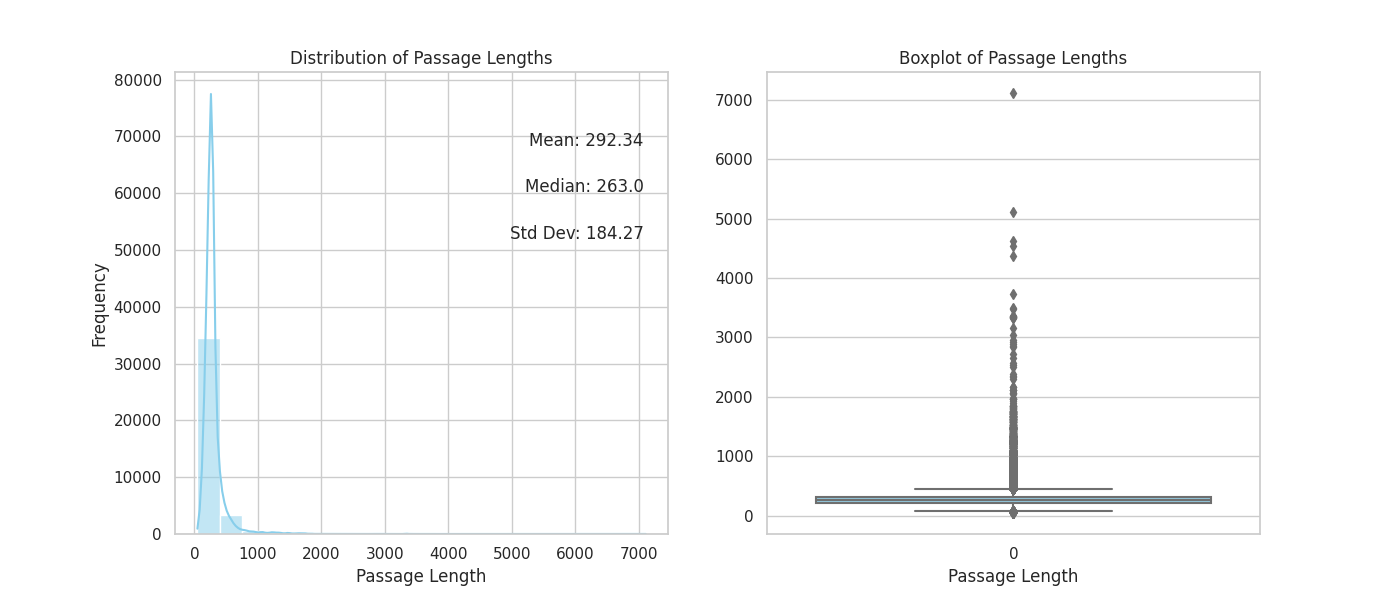
\includegraphics[width=\textwidth]{Grafiken/Statistiken/IndexGerman_Passage_Length_Statistics_old.png}
    \caption{Passage Length Distribution of the German \gls{er} Dataset before Filtering}
    \label{fig:er-german-passage-length-old}
\end{figure}

In Step (3), every passage and all in Step (5) generated questions of the German and English \gls{er} dataset are translated using the Google Translate API. This creates a two more dataset in addition to the existing two, which are directly based on the document's language.

The final Step (4) toward the \textit{knowledge source} is the index creation. To simplify the later \gls{rag} system, the decision was made not to use a hierarchical index structure. However, this could lead to problems when users need to find specific information within one document and want to perform metadata-filtering. To address this, all passages have the title of the document from which they were extracted concatenated to them in the following way:

\begin{quotation}
    \{passage\} + \texttt{ - } + \{documentName\}
\end{quotation}

This approach enables the retriever and reader to identify passages and their corresponding documents in a single step, as opposed to hierarchical index implementations that necessitate multiple steps and potentially multiple databases for embeddings and metadata of the passages. This method has been chosen because, in this use-case, the only utilized and easy extractable metadata of a document is a documents title (e.g., \textit{Examination Regulation for the Master Data and Computer Science}, with some even including the date). Other use-cases may require more complicated appraoches. For the translated datasets, the document name will be translated, as described in Step (3).

\textbf{Data Augmentation:} Step (5) of the extraction pipeline involves data augmentation. For \textit{Question Generation} based on a given passage, the few-shot approach from \textit{PROMPTAGATOR} \cite{dai_promptagator_2022} has been employed. For the English \gls{er} dataset, the following prompt is used to generate a question, given a passage and $i$ examples:

\begin{quote}
   \texttt{System Prompt:}\\
    \texttt{You are an assistant generating one question given a context. Please start your generated question with the indicator 'Generated Question:' Here are some examples:} \\
    for example in examples:\\
    \hspace*{1cm}\{i\}\texttt{-Example:} \\
    \hspace*{1cm}\texttt{Context:} \{passage\} \\
    \hspace*{1cm}\texttt{Generated Question:} \{question\} \\ \\
    \texttt{User:} \\
    \texttt{Generate the question based on the following context:}\\
    \{passage\}
    \label{prompt:system-prompt-data-generation}
\end{quote}

The snippet in the System Prompt is looped four times to accommodate the number of examples. The examples represent different question types, which themeself indicate different answer types, in order to add some variety to the generated data. The used examples can be found in the appendix \ref{ref:appendixA-data-augmentation-few-shot-prompt}. The Prompt is generally designed to be used with a chat fine-tuned model, as it showed better results in a qualitative evaluation. For English question generation, the \textit{Llama2-7B-Chat-GPTQ}\footnote{\url{https://huggingface.co/TheBloke/Llama-2-7b-Chat-GPTQ}} is employed. It's a quantized version of the original Llama2-7B-Chat Model by Meta \cite{touvron_llama_2023}. For the German \gls{er}, the same prompt translated to English is used. For the German tasks, the \textit{Leo-Hessianai-7B-Chat-GPTQ}\footnote{\url{https://huggingface.co/TheBloke/leo-hessianai-7B-chat-GPTQ}} model is used, which is a quantized version of a German language fine-tuned Llama2-7B-Chat Model \cite{pluster_leolm_2023}.

It's worth noting that the English Llama2-7B-Chat was capable of directly understanding the system prompt and generating questions with the indicator \texttt{Generated Question}, which made using the generated text easier. However, the German \gls{llm} struggled with this Few-Shot task and often generated multiple responses that didn't start with the indicator \texttt{Generierte Frage}. Additionally, the model sometimes included answers after the questions. To extract the single question from the generated text in the German \gls{llm} output, the text is cropped after a \texttt{:} and \texttt{?}, so the string enclosed by these characters is used as the question for a given passage. 

The choice of Llama2-based models was based on their new state-of-the-art results in multiple benchmarks, as demonstrated by these models in the open-source \gls{llm} niche \cite{touvron_llama_2023}. Additionally, the work of Plüster et al. \cite{pluster_leolm_2023} on LeoLama opens the opportunity to compare the performance of German and English \gls{llm}s from the same family.

For \textit{Answer Generation}, the previously generated questions per passage are utilized. The \gls{llm} is prompted in the following manner:

\begin{quote}
    \texttt{System Prompt:}\\
    \texttt{You are an assistant who generates gold answers for a given question and context.}\\
    \texttt{User:}\\
    \texttt{Generate the answer based on the following question and context:}\\
    \texttt{Question:} \{question\} \\
    \texttt{Context:} \{passage\}
\end{quote}

This prompt was applied in both German and English to generate gold answers for all datasets. A random selection of 2000 samples was drawn from the original German and English \gls{er} datasets and their translated versions, resulting in four selections of 2000 question-context pairs each\footnote{This sampling approach will also be employed later to mitigate the costs associated with the OpenAI API}. On this smaller selection, \textit{gpt-3.5-turbo} was employed with the mentioned prompt to generate high-quality question-context-answer triples. Additionally, \textit{leo-hessianai-7B-chat-GPTQ} and \textit{Llama2-7B-Chat-GPTQ} (See Section \ref{subsec:reader-impl}) were used to generate gold answers over the entire dataset. The sampled high-quality gold-answer sets will be employed in Section \ref{subsec:reader-results} to compare the gold-answer generation quality of the smaller models against the larger \textit{gpt-3.5-turbo} model. In order to extend the triples to contain not only the correct context, but also other high probable contexts per question, the large \gls{dpr} retriever (See Section \ref{subsec:retriever-impl}) was used per triple to retrieve the top 10 passages. Those were appended to the context of the triple. This will be used in the reader evaluation later.

\subsection{Retriever}
\label{subsec:retriever-impl}

The implemented retrievers can be found in Figure \ref{fig:retriever-implementation}. Given the limited availability of (synthetic) data suitable for fine-tuning, the decision was made to exclusively utilize top-performing \gls{ood} zero-shot retrievers. Fine-tuning a model on such a small dataset could lead to a high risk of overfitting. To assess retriever performance, the synthetic dataset will be used for benchmarking. Among the top-performing retrievers from the BEIR benchmarks, the following three retrievers have been choosen:

\begin{enumerate}
    \item \textbf{BM25:} This employs the standard lexical-based best match algorithm with hyperparameters $k_1=1.5$, $b=0.75$, and $\epsilon=0.25$. It is implemented using the open-source project \textit{rank-bm25} \footnote{\url{https://github.com/dorianbrown/rank_bm25}}.
    \item \textbf{BM25 + CE:} This uses a BM25 retriever in combination with a Cross-Encoder re-ranker, which serves as the baseline established in BEIR \cite{thakur_beir_2021}. This combination continues to perform as the state-of-the-art. The Cross-Encoder utilized is the same as the one in the BEIR baseline implementation: \textit{ms-marco-MiniLM-L-6-v2} \cite{wang_minilm_2020}, specifically the implementation provided on Hugging Face \footnote{\url{https://huggingface.co/cross-encoder/ms-marco-MiniLM-L-6-v2}}. It has close to 17 million parameters. For German indices, a German version of \textit{ms-marco-MiniLM-L-6} is used: \textit{ms-marco-MiniLM-L-6-en-de-v1} \footnote{\url{https://huggingface.co/cross-encoder/msmarco-MiniLM-L6-en-de-v1}}.
    \item \textbf{Large DPR:} For the large \gls{dpr}, the embedding model from OpenAI, \textit{text-embedding-ada-002} \footnote{\url{https://platform.openai.com/docs/models/embeddings}}, is employed. The parameter size of this model is estimated to be around 350 million parameters\cite{muennighoff_sgpt_2022}\footnote{As OpenAI does not publicly provide information on their model specs, there exist only estimates.}.
\end{enumerate}

These retrievers have been implemented and evaluated based on the synthetic data, and the results are presented in Section \ref{sec:results}.

\begin{figure}
    \centering
    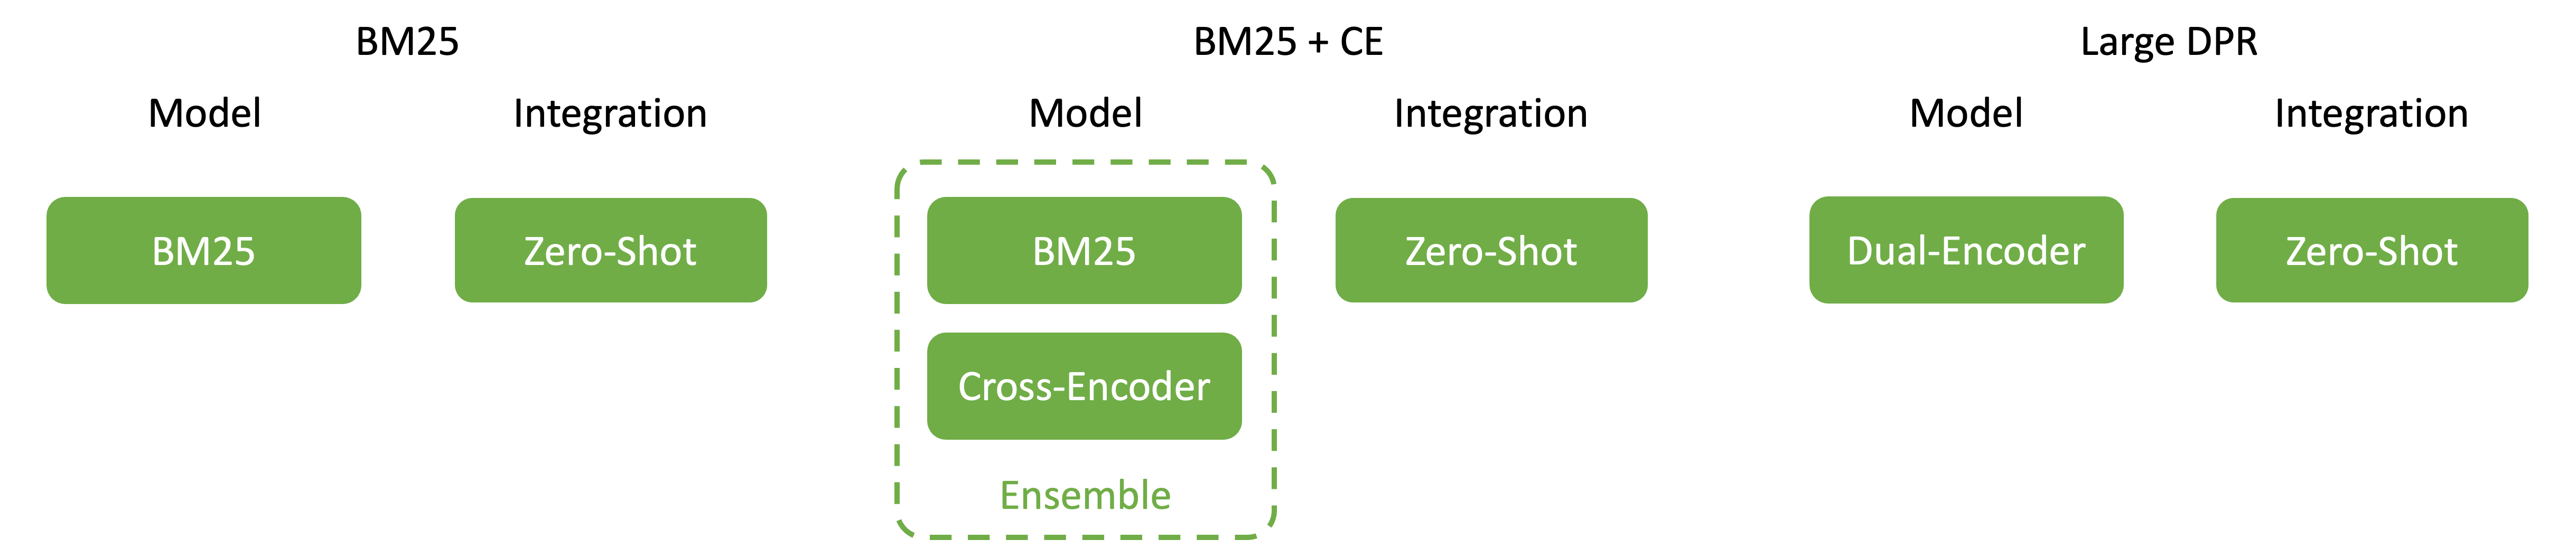
\includegraphics[width=\textwidth]{Grafiken/Evaluation/retriever_implemented.png}    
    \caption{Implemented Retrievers}
    \label{fig:retriever-implementation}
\end{figure}

\subsection{Reader}
\label{subsec:reader-impl}

The implemented readers can be found in Figure \ref{fig:reader-implementation}. Due to the limited hardware resources and high-quality data, the decision was made to only use zero-shot pre-trained \glspl{llm}s for the reader component and not fine-tune any. The following readers have been chosen:

\begin{enumerate}
    \item \textbf{gpt-3.5-turbo:} GPT 3.5 Turbo is part of the OpenAI chat completion family\footnote{\url{https://platform.openai.com/docs/models/gpt-3-5}}. Details on the parameters are not available. However, the latest published research by OpenAI indicates 175B parameters for the model on which GPT 3.5 Turbo was built. In general, the model is an \gls{llm} trained using human feedback on chat-like completion tasks \cite{ouyang_training_2022}. It accepts up to 4,096 tokens as input.
    \item \textbf{Llama2-7B-Chat-GPTQ:} This is a quantized version of the original Llama2-7B-Chat Model by Meta \cite{touvron_llama_2023}. The model is an \gls{llm} trained on chat-instruction datasets \cite{ouyang_training_2022}. The model is available on Hugging Face\footnote{\url{https://huggingface.co/TheBloke/Llama-2-7b-Chat-GPTQ}}. The model is quantized using GPTQ \cite{muennighoff_sgpt_2022}. However, the provider did not report any benchmarks indicating the accuracy drop of the GPTQ version compared to the original. It accepts up to 4,096 tokens as input.
    \item \textbf{leo-hessianai-7B-chat-GPTQ:} \textit{Linguistisch Erweitertes Offenes Language Model} (LeoLM) is a German tasks fine-tuned version of the original Llama2-7B-Chat model. The original Llama2 is fine-tuned on a large corpus of German language texts, and multiple adjustments are applied to overcome the problem of forgetting. This results in a maximum input token length of 8,000 tokens. In addition to original German chat instruction-based datasets, automatic translated English benchmark datasets are used as well. Benchmarking results indicate an increase in German language capabilities while maintaining English language task performance \cite{pluster_leolm_nodate}.
\end{enumerate}

Generally, \textbf{gpt-3.5-turbo} acts as a higher-end benchmark. It is a state-of-the-art \gls{llm} with high popularity in the media and developer community. \textbf{Llama2-7B-Chat-GPTQ} should be a hardware resource-efficient alternative pre-trained model, especially the quantized version that can run on consumer hardware. \textbf{leo-hessianai-7B-chat-GPTQ} is representative of a German native model, providing further insights into language dependencies and the performance of \gls{llm}s, as the use case involves multiple indices in German and English.

Additional approaches, such as evaluating different fine-tuning strategies, have been excluded, as they would open up a vast problem space that cannot be adequately covered within the scope of this thesis. Therefore, the thesis predominantly concentrates on a comprehensive \gls{poc} to demonstrate and evaluate one possible implementation approach of the framework introduced in Section \ref{chap:main}, utilizing the mentioned \gls{llm}s.

However, to address specific questions in the evaluation (See Section \ref{subsec:reader-results}), such as \textit{How many contexts can the model receive and still determine the correct answer?}, the reader prompt was structured to accept multiple contexts as inputs to the question:

\begin{quote}
    \texttt{System Prompt:} \\
    \texttt{You are an assistant helping a student with examination regulations of the Heidelberg University. Generate a concise answer based on the provided contexts. If the answer isn't in the contexts, state 'I can't answer this question'. If there's ambiguity, ask clarifying questions.} \\
    \{previous chat history\}\\
    \texttt{User:} \\
    \texttt{Please generate an answer for the following question:} \\
    \{question\} \\
    \texttt{Use the following contexts:} \\
    for context in contexts: \\
    \hspace*{1cm}\{context\} \\
    \texttt{Assistant:} \\
\end{quote}

This prompt is applied consistently across all models. In cases where the model is applied on a German dataset, a German version of this prompt is utilized.


\begin{figure}
    \centering
    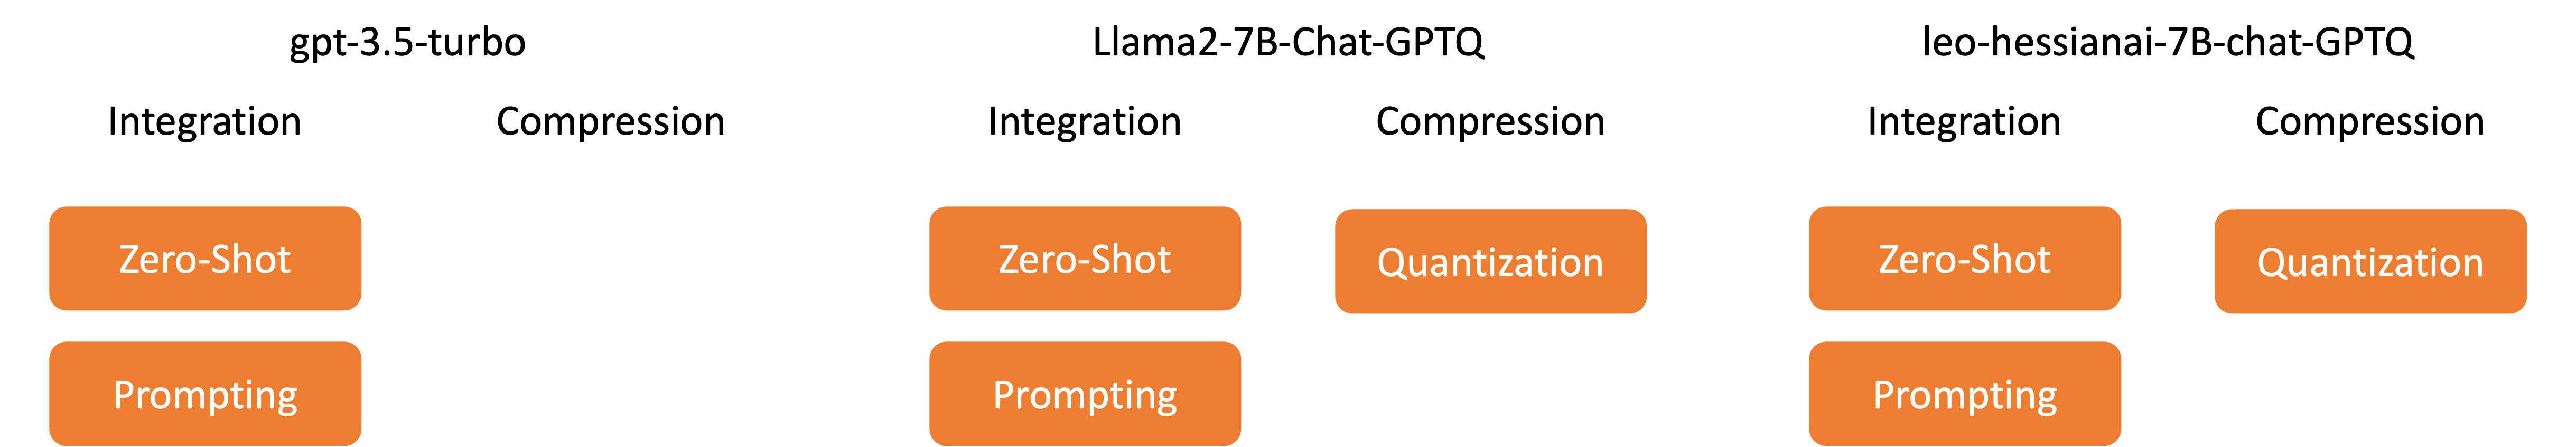
\includegraphics[width=\textwidth]{Grafiken/Evaluation/reader_implemented.png}
    \caption{Implemented Readers}
    \label{fig:reader-implementation}
\end{figure}

\subsection{CQU}
\label{subsec:cqu-impl}

Similar to the Reader and Retriever components, the implementation of the \gls{cqu} component can be observed in Figure \ref{fig:cqu-implementation}. Generally, the \gls{cqu} component utilizes a \gls{llm} for query rewriting based on the last-$k$ turns of the conversation history. $k$ is thereby not a fixed value, but rather the number of tokens for every turn will be calculated and only the last-$k$ turns until which the prompt does not overstep the token limit of the model, will be used. This follows the \textit{Rewriting Prompt} implementation by Mao et al. \cite{mao_large_2023}. Their work demonstrated that \gls{llm}s can achieve state-of-the-art benchmarks for \gls{cqu}. Mao et al. also explored other approaches to prompting beyond simple rewriting, which, while outperforming simple rewrite, are only applicable to \gls{dpr}-based retrievers.

\begin{figure}[H]
    \centering
    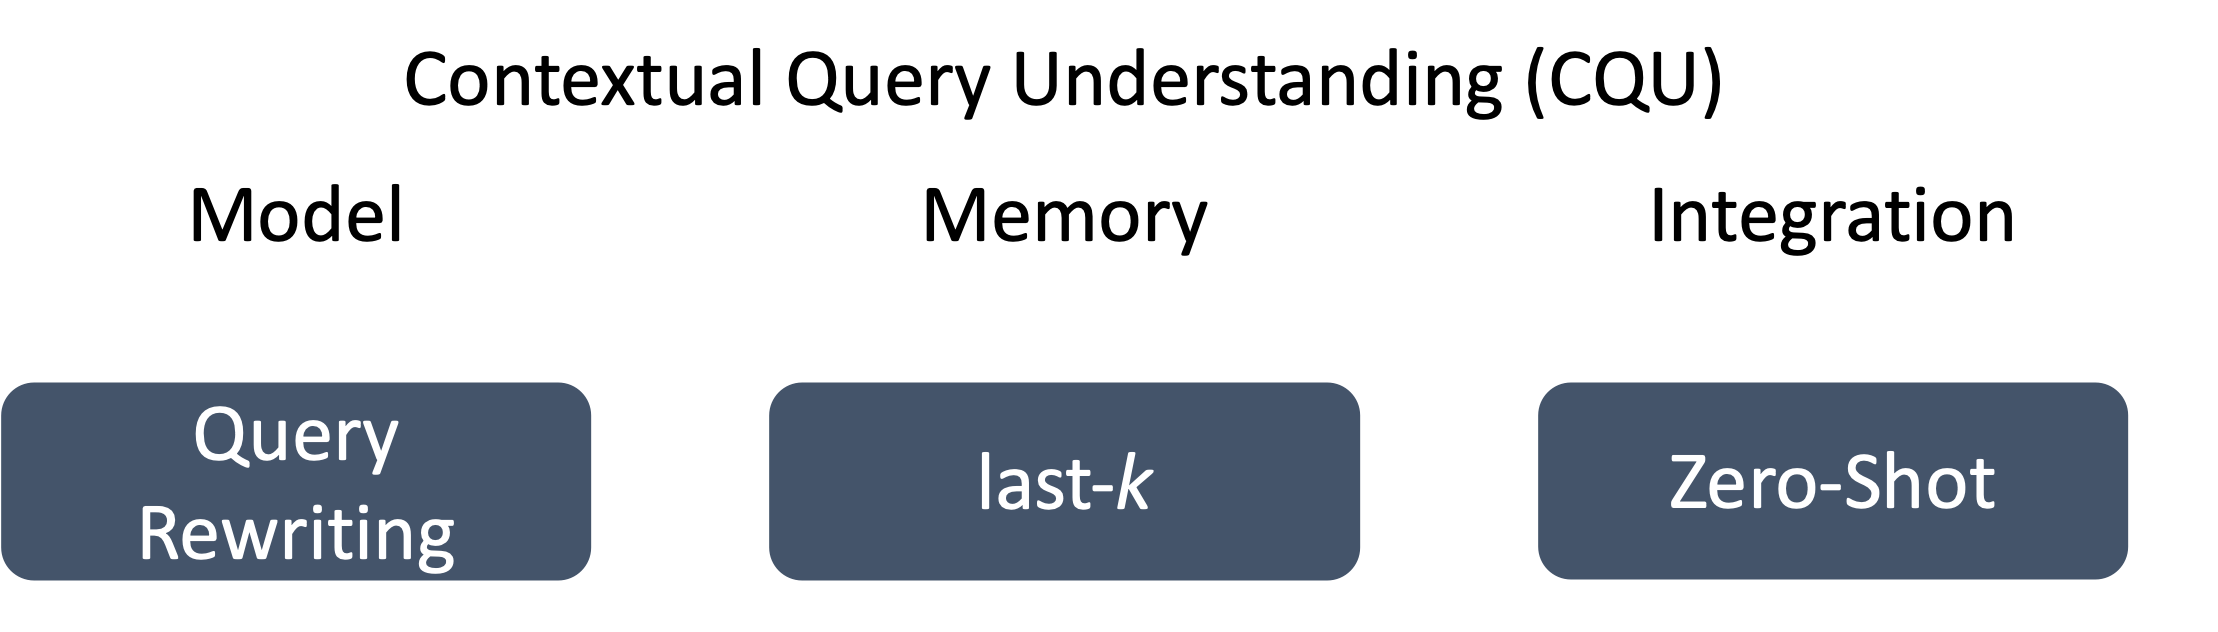
\includegraphics[width=0.6\textwidth]{Grafiken/CQU_Implementation.png}
    \caption{Implemented CQU}
    \label{fig:cqu-implementation}
\end{figure}

The simple rewrite prompt is implemented as follows:

\begin{quote}
    \texttt{System Prompt:}\\
    \texttt{As an assistant, you're tasked to decontextualize and reformulate the current question considering a multi-turn information-seeking dialogue. Please provide only the rewritten question after 'Rewrite:'. It will be used for passage retrieval. Here are some examples:} \\
    for example in example:\\
    \hspace*{1cm}\{example\}-\texttt{Example:} \\
    \hspace*{1cm}for turn in turns:\\
    \hspace*{1cm}\hspace*{1cm}\{turn\}-\texttt{Turn:} \\
    \hspace*{1cm}\hspace*{1cm}\texttt{Question:} \\
    \hspace*{1cm}\hspace*{1cm}\{question\} \\
    % \hspace*{2cm}\texttt{Rewrite:} \\
    % \hspace*{2cm}\{rewrite\} \\
    \hspace*{1cm}\hspace*{1cm}\texttt{Answer:} \\
    \hspace*{1cm}\hspace*{1cm}\{answer\} \\
    \hspace*{1cm}\texttt{Question:} \\
    \hspace*{1cm}\{question\} \\
    \hspace*{1cm}\texttt{Rewrite:} \\
    \hspace*{1cm}\{rewritten last user question\} \\
    \{previous chat history\} \\
    \texttt{User:}\\
    \texttt{Please rewrite the following question given this conversation history:}\\
    % for turn in turns - 1:\\
    % \hspace*{1cm}\{turn\}-\texttt{Turn:}\\
    % \hspace*{1cm}\texttt{Question:} \\ 
    % \hspace*{1cm}\{question\}\\
    % \hspace*{1cm}\texttt{Answer:}\\ 
    % \hspace*{1cm}\{answer\}\\
    \texttt{Question:}\\
    \{question\}\\
    \texttt{Rewrite:}\\
\end{quote}

In terms of models, the same models as for the Reader component will be utilized: \textit{Llama2-7B-Chat-GPTQ} for English conversations and \textit{leo-hessianai-7B-chat-GPTQ} for German conversations. The \gls{cqu} component itself will not be evaluated since there is no dataset available. For evaluations of this approach on other datasets and \gls{llm}s, the reader is referred to the work of Mao et al. \cite{mao_large_2023}.

\section{Experimental Results}
\label{sec:results}

This section evaluates the implemented system and the introduced framework, using metrics introduced in Section \ref{sec:metrics}. The evaluation covers the following components: \textit{Extraction}, especially synthetic data generation (Section \ref{subsec:data-augmentation-quality}), \textit{Retriever} (Section \ref{subsec:retrieval-results}), \textit{Reader} (Section \ref{subsec:reader-results}), and the complete \gls{convqa} system (Section \ref{subsec:convqa-results}). The evaluation is based on the synthetic dataset described in Section \ref{subsec:index}, generated from the dataset introduced in Section \ref{sec:data}.

\subsection{Evaluation Limitations}
\label{subsec:data-augmentation-quality}

The outlined limitations primarily pertain to the Reader Evaluation. The Retriever Evaluation should be minimally affected, mainly by the usefulness of the generated questions. This section serves as a guide for future work, particularly when dealing with synthetic data generation. For more robust insights into \gls{rag} and the reader component in a conversational scenario, refer to Section \ref{subsec:convqa-results}, which is based on real-world data rather than synthetically generated data.

\vspace{\baselineskip}
\noindent\textbf{LLM Performance:} As detailed in Section \ref{subsec:index}, the two main indices, namely \textit{indexEnglish} and \textit{indexGerman}, are based on the corresponding \gls{er}s. During the generation of the question-context datasets, qualitative issues arose when using \textit{leo-hessianai-7B-chat-GPTQ}. As indicated by System Prompt \ref{prompt:system-prompt-data-generation}, the model was prompted to start the generated answer after a defined indication text. In multiple cases, the German model \textit{leo-hessianai-7B-chat-GPTQ} was unable to fulfill this request, necessitating post-processing as described in Section \ref{subsec:index}. This issue was not present when using the English model \textit{Llama2-7B-Chat-GPTQ}. This observation highlights a zero-shot performance gap between the English model \textit{Llama2-7B-Chat-GPTQ} and the German model \textit{leo-hessianai-7B-chat-GPTQ}. Consequently, the subsequent evaluations will concentrate on the \textit{indexEnglish} and \textit{translated-indexEnglish} datasets.

%one line skip
\vspace{\baselineskip}
\noindent\textbf{Gold-Answer-Generation Performance:} The \textit{Human-based} reader's accuracy evaluation (Table \ref{tab:human-reader-evaluation}) shows a low rate of correct gold answers, approximately 22.25\%. The main reason for incorrectness is hallucination by smaller \gls{llm}s, leading to mostly incorrect gold answers. This impacts the performance of different evaluation metrics for the reader. The \textit{F1-BERTscore} operates only on the gold answer $\hat{a}$ and the predicted answer $a'$, potentially lacking sufficient insights. In contrast, the \textit{LLM-based} accuracy considers a triplet of question $q$, gold answer $\hat{a}$, and predicted answer $a'$, making it more robust to hallucination within gold answers. Across all models and indices, there is a gap of approximately 20.4\% between \textit{Human-based} and \textit{LLM-based} results. The \textit{short} versions of the indices, which use gold answers generated by \textit{gpt-3.5-turbo} with less hallucination, show a gap of 9.11\% when filtered for only useful gold answers. Therefore, the evaluation will focus on the \textit{short} versions of the indices for the reader.

\vspace{\baselineskip}
\noindent\textbf{Generated Question Usefulness:} As observed in Section \ref{subsec:index}, the approach for synthetic question generation aims to create various question types, including extractive and conceptual questions. However, the \textit{Human-based} Evaluation reveals that only 51.25\% of the generated questions are extractive, meaning they can be answered with information from the passage they are based on. This poses a significant challenge for automatically evaluating the reader and retriever components, as only a portion of the question-context tuples can be assessed in such constellations. Others may not make sense as the desired information might not be in the answer or even provided in the knowledge base. Despite this, in Figure \ref{fig:retriever-performance-bm25-vs-dpr}, retrievers show diminishing returns in performance improvement at approximately $k = 300$, reaching \gls{hr}s between 0.71 and 0.96. However, for future work, the entire evaluation pipeline using synthetic data must be reconsidered, especially for evaluating complex question types.

\vspace{\baselineskip}
\noindent\textbf{Negative Rejection Evaluation:} The chosen approach to automatically evaluate negative rejection, as described in Section \ref{subsec:reader-results}, faces two major challenges. Firstly, multiple passages are identical across the knowledge base, rendering the removal of the gold passage from the evidence set redundant. Secondly, as discussed in the \textbf{Generated Question Usefulness} section, the removal of the gold passage may still leave sufficient information in the evidence set to answer the question. This does not create an ideal scenario for evaluating negative rejection capabilities. A more suitable approach would be to manually generate a set of questions that are unanswerable by the knowledge base and then evaluate the models on this set. However, this approach may not be feasible with synthetic data.

\vspace{\baselineskip}
\noindent\textbf{BLUE and ROUGE Metrics:} The applicability of \textit{BLUE} and \textit{ROUGE} metrics in the context of generative readers for question answering needs to be questioned. Applying these metrics to evaluate the reader in the given setup leads to random results. This is because these metrics are designed to determine a vocabulary-based overlap between two texts, which is only applicable in the case of extractive readers, not generative readers as used in \gls{rag}.


\subsection{Retrieval Results}
\label{subsec:retrieval-results}

The evaluation based on the described metrics (See Section \ref{sec:metrics}) delivers multiple insights:


% TODO: Needs correction as soon as benchmark is done
\begin{enumerate}
    \item Overall, the out-of-domain zero-shot performance of the large \gls{dpr} outperforms BM25 for all $k$-values, indices and languages. This can be observed in Figure \ref{fig:retriever-performance-bm25-vs-dpr}.
    \item The ensemble of \textit{BM25-CE} outperforms the regular \textit{BM25} retriever for three out of four indices (all except for the \textit{indexGerman}) when considering small values of $k$. Figure \ref{fig:retriever-performance-bm25-vs-bm25-ce-mrr} compares the \gls{mrr} between the standard \textit{BM25} retriever and \textit{BM25-CE} retriever with the BM25 $k$-value set to 500. As the \textit{Reader} component ideally takes as small a set of passages as possible as input, the \textit{BM25-CE} retriever is the better choice. The internal $k$-value of the first stage \textit{BM25} retriever can be as large as possible, as it only improves the performance of the Re-Ranker. However, depending on the dataset and use-case, an increasing $k$-value may not necessarily improve performance, as it seems to exist an upper performance limit in the cross-encoder component.
    \item Figure \ref{fig:retriever-performance-bm25-ce-k} compares different \textit{BM25-CE} Re-Ranker settings over the \textit{indexEnglish} index. It can be observed, that an increase in the first-stage Retriever's $k$-value does at some point not longer increase the performance of the Re-Ranker. This is true for the \gls{mrr} and \gls{hr}.
    
    \item In the comparison of \textit{BM25} and \textit{\gls{dpr}} retrievers for different languages, the final choice of the \textit{Retriever} component should consider the best \gls{mrr} value for English and German datasets for $k \leq 10$. Figure \ref{fig:retriever-performance-best-retriever} compares \textit{BM25-CE-500} with the large \textit{\gls{dpr}} retriever over all datasets. The \gls{dpr} retriever significantly outperforms the \textit{BM25-CE-500} retriever for all datasets, indicating a high multi-language zero-shot performance of the \textit{text-embedding-ada-002} model by OpenAI. Nevertheless, considering the diffference in parameters (350 million vs. 17 million), the \textit{BM25-CE-500} retriever is a good alternative.
\end{enumerate}

\begin{figure}[h]
    \centering
    \begin{subfigure}{.5\textwidth}
        \centering
        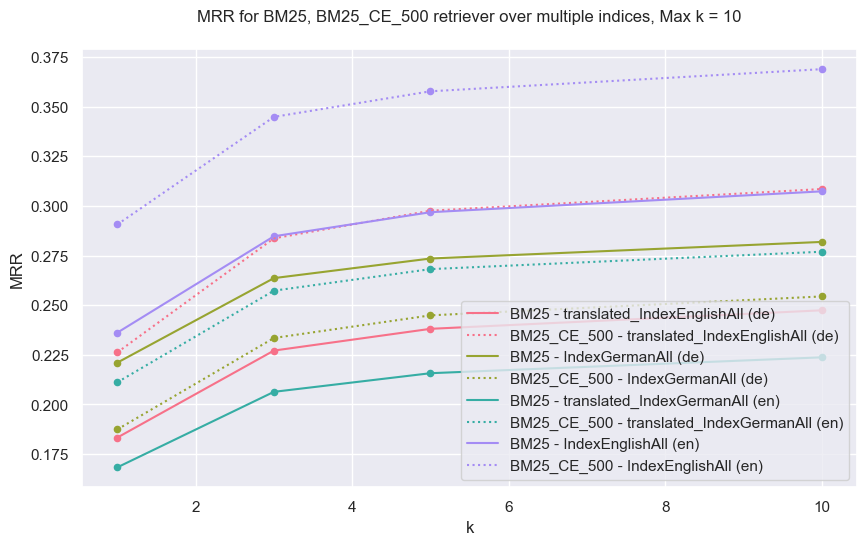
\includegraphics[width=\linewidth]{Grafiken/Evaluation/Data_Generation/BM25_vs_BM25_CE_MRR.png}
        \captionsetup{width=.9\linewidth}
        \caption{BM25 and BM25-CE MRR performance for $k = 10$}
        \label{fig:retriever-performance-bm25-vs-bm25-ce-mrr}
    \end{subfigure}%
    \begin{subfigure}{.5\textwidth}
        \centering
        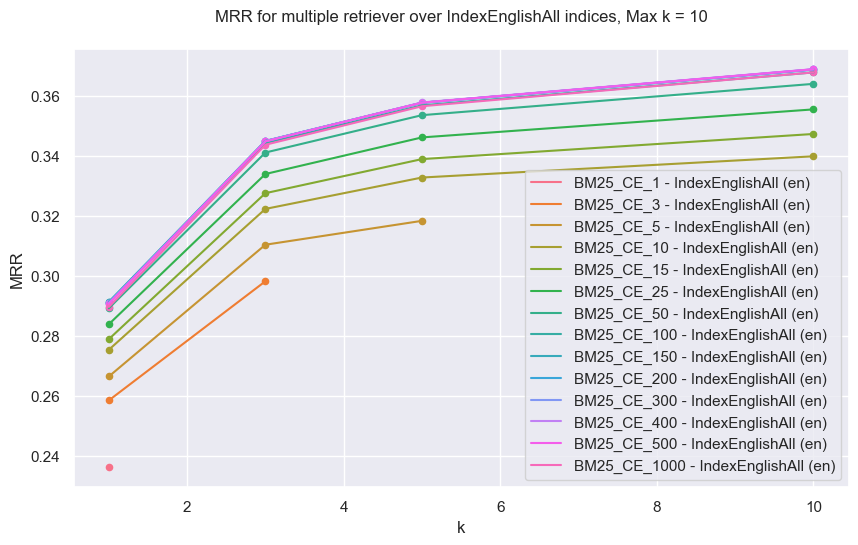
\includegraphics[width=\linewidth]{Grafiken/Evaluation/Data_Generation/BM25_CE_k.png}
        \captionsetup{width=.9\linewidth}
        \caption{BM25-CE HR performance for different BM25 $k$-values}
        \label{fig:retriever-performance-bm25-ce-k}
    \end{subfigure}
    \begin{subfigure}{.5\textwidth}
        \centering
        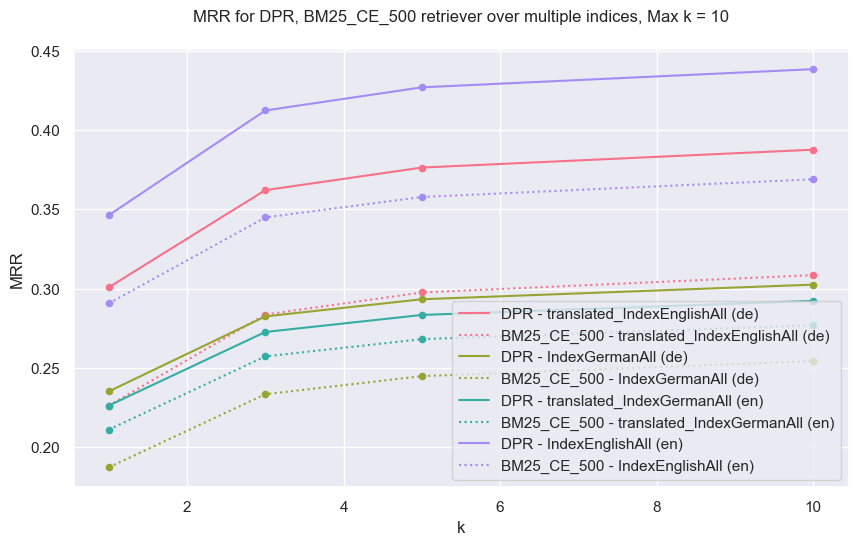
\includegraphics[width=\linewidth]{Grafiken/Evaluation/Data_Generation/best_retriever.png}
        \captionsetup{width=.9\linewidth}
        \caption{BM25-CE and DPR MRR performance for $k = 10$}
        \label{fig:retriever-performance-best-retriever}
    \end{subfigure}%
    \begin{subfigure}{.5\textwidth}
        \centering
        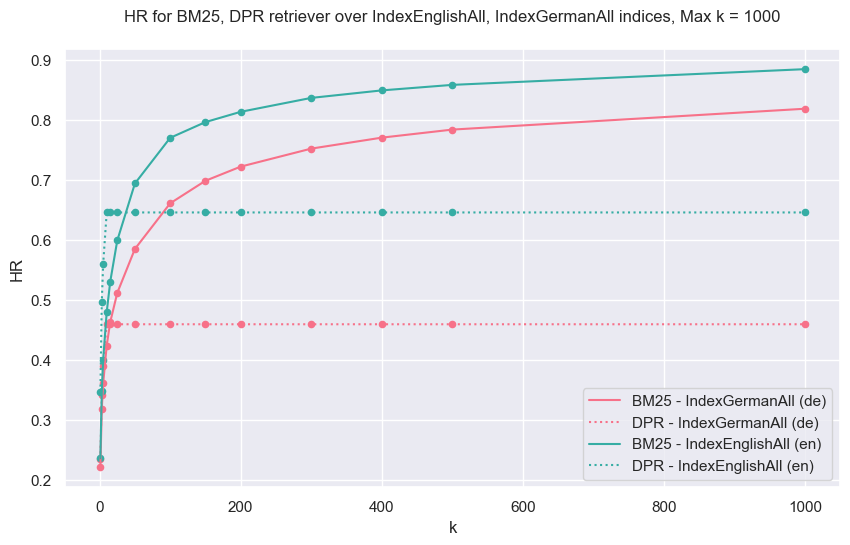
\includegraphics[width=\linewidth]{Grafiken/Evaluation/Data_Generation/BM25_DPR_1000.png}
        \captionsetup{width=.9\linewidth}
        \caption{BM25 and Large DPR performance comparison for $k = 1000$}
        \label{fig:retriever-performance-bm25-vs-dpr}
    \end{subfigure}
    \caption{Multiple Retriever Performance Comparisons}
    \label{fig:retriever-performance}
\end{figure}

% \begin{figure}
%     \centering
%     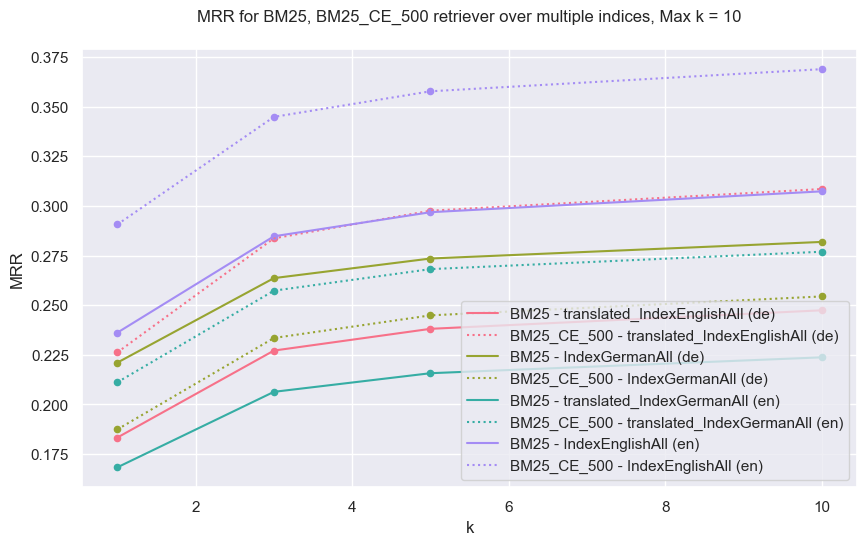
\includegraphics[width=\textwidth]{Grafiken/Evaluation/Data_Generation/BM25_vs_BM25_CE_MRR.png}
%     \caption{BM25 and BM25-CE MRR perfromance for $k = 10$}
%     \label{fig:retriever-performance-bm25-vs-bm25-ce-mrr}
% \end{figure}

% \begin{figure}
%     \centering
%     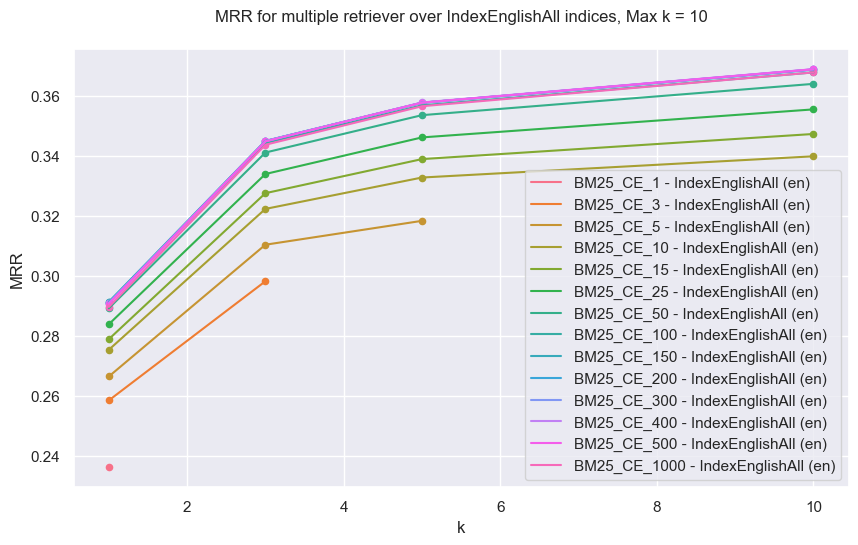
\includegraphics[width=\textwidth]{Grafiken/Evaluation/Data_Generation/BM25_CE_k.png}
%     \caption{BM25-CE HR perfromance for different BM25 $k$-values}
%     \label{fig:retriever-performance-bm25-ce-k}
% \end{figure}

% \begin{figure}
%     \centering
%     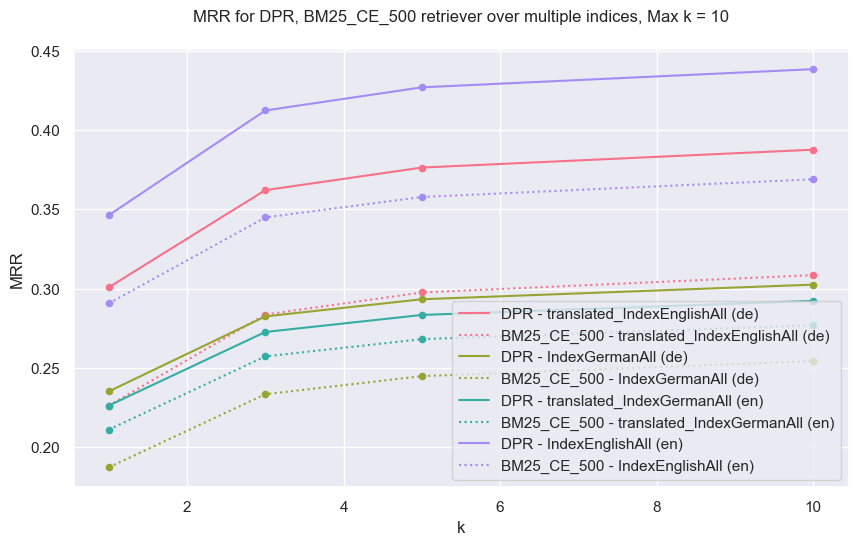
\includegraphics[width=\textwidth]{Grafiken/Evaluation/Data_Generation/best_retriever.png}
%     \caption{BM25-CE and DPR MRR perfromance for $k = 10$}
%     \label{fig:retriever-performance-best-retriever}
% \end{figure}

% \begin{figure}
%     \centering
%     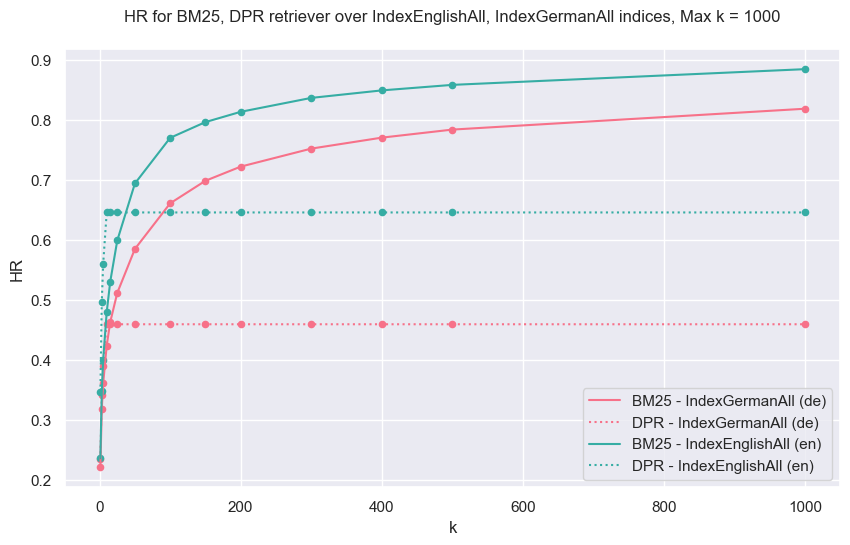
\includegraphics[width=\textwidth]{Grafiken/Evaluation/Data_Generation/BM25_DPR_1000.png}
%     \caption{BM25 and Large DPR performance comparison for $k = 1000$}
%     \label{fig:retriever-performance-bm25-vs-dpr}
% \end{figure}

The influence of the Retriever component will be further evaluated in Section \ref{subsec:convqa-results}. Here the bottlenecks of the system will be identified and discussed. A full set of evaluation results can be found in the tables in Appednix \ref{ref:appendixA-evaluation-retriever}.

% \begin{figure}
%     \centering
%     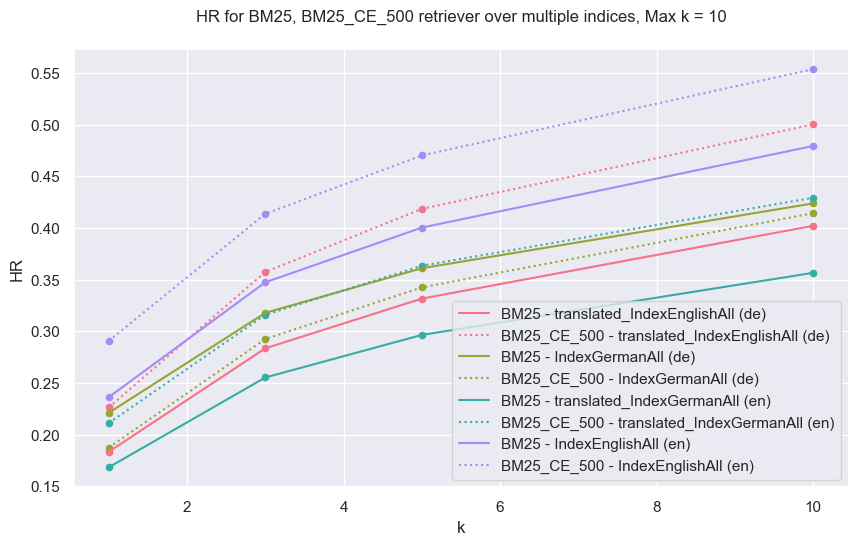
\includegraphics[width=\textwidth]{Grafiken/Evaluation/Data_Generation/BM25_vs_BM25_CE.png}
%     \caption{BM25 and BM25-CE HR perfromance for $k = 10$}
%     \label{fig:retriever-performance-bm25-vs-bm25-ce-hr}
% \end{figure}

\subsection{Reader Results}
\label{subsec:reader-results}


The evaluation of the Reader is based on the metrics introduced in Section \ref{sec:metrics}. Some adjustments have been made as follows: Firstly, whenever \textit{gpt-3.5-turbo} is evaluated on a dataset, it is assessed on a random sample of 1,000 elements based on that dataset. Secondly, when calculating the \gls{llm}-based accuracy, it is computed on a random sample set of 1000 elements of a model's predictions. These adjustments aim to mitigate the costs associated with the OpenAI API. Thirdly, two separate datasets have been generated based on the four already introduced indices: \textit{indexEnglish}, \textit{indexGerman}, \textit{translated indexEnglish}, and \textit{translated indexGerman}. The \textit{short} version of the datasets corresponds to 2,000 random samples, where \textit{gpt-3.5-turbo} is used to generate the gold-answers in the data augmentation stage. The \textit{filtered} version of the datasets drops question-context pairs if the gold-passage is not included in the evidence set of the \gls{dpr} retriever with $k = 1,000$ and generates the gold-answers using \textit{Llama2-7B-Chat-GPTQ} for \textit{indexEnglish} and \textit{translated indexGerman}, and \textit{leo-hessianai-7B-chat-GPTQ} for \textit{indexGerman} and \textit{translated indexEnglish}. In order to test the \textit{Negative Rejection}, with a randomness of 20\% the correct passage was removed from the evidence set of the \gls{dpr} retriever. Those evaluation datasets will be refered to as \textit{dropped} datasets. 

Table \ref{tab:human-reader-evaluation} presents the evaluation results for the reader component based on filtered versions of the datasets. Specifically, the \textit{gpt-3.5-turbo} model is assessed on the \textit{indexEnglish} and \textit{translated indexEnglish} datasets, while the \textit{leo-hessianai-7B-chat-GPTQ} and \textit{Llama2-7B-Chat-GPTQ} models are evaluated on the \textit{indexGerman} and \textit{translated indexGerman} datasets. The Cohen's Kappa coefficient indicates a moderate agreement between the two evaluators, scoring $0.72$.

\begin{table}[h]
    \renewcommand{\arraystretch}{1.1}
    \resizebox{\textwidth}{!}{%
    \begin{tabular}{p{0.35\textwidth}p{0.1\textwidth}cccccc}
    \hline
    \multicolumn{2}{l}{\multirow{2}{*}{Index}}                              & \multicolumn{2}{c}{\textit{gpt-3.5-turbo}}                                                                            & \multicolumn{2}{c}{\textit{leo-hessianai-7B-chat-GPTQ}}                                                                 & \multicolumn{2}{c}{\textit{Llama2-7B-Chat-GPTQ}}                                                   \\ \cline{3-8} 
    \multicolumn{2}{l}{}                                                    & accuracy                  & accuracy qat*                                                              & accuracy                  & accuracy qat*                                                                 & accuracy                  & accuracy qat*                                            \\ \hline
    \multirow{2}{*}{IndexEnglish}            & \multicolumn{1}{c|}{all}     & \multicolumn{1}{c|}{0.68} & \multicolumn{1}{c|}{\begin{tabular}[c]{@{}c@{}}1.0\\ (34.5/10)\end{tabular}} & \multicolumn{2}{c|}{\multirow{2}{*}{-}}                                                                   & \multicolumn{1}{c|}{0.24} & \begin{tabular}[c]{@{}c@{}}0.3571\\ (16/14)\end{tabular} \\ \cline{2-4} \cline{7-8} 
                                             & \multicolumn{1}{c|}{dropped} & \multicolumn{1}{c|}{0.56} & \multicolumn{1}{c|}{\begin{tabular}[c]{@{}c@{}}0.675\\ (40)\end{tabular}}  & \multicolumn{2}{c|}{}                                                                                     & \multicolumn{1}{c|}{0.52} & \begin{tabular}[c]{@{}c@{}}0.5334\\ (30)\end{tabular}    \\ \hline
    \multirow{2}{*}{translated IndexEnglish} & \multicolumn{1}{c|}{all}     & \multicolumn{1}{c|}{0.62} & \multicolumn{1}{c|}{\begin{tabular}[c]{@{}c@{}}0.9545\\ (39/10.5)\end{tabular}} & \multicolumn{1}{c|}{0.2}  & \multicolumn{1}{c|}{\begin{tabular}[c]{@{}c@{}}0.2367\\ (13/10)\end{tabular}} & \multicolumn{2}{c}{\multirow{2}{*}{-}}                                               \\ \cline{2-6}
                                             & \multicolumn{1}{c|}{dropped} & \multicolumn{1}{c|}{0.58} & \multicolumn{1}{c|}{\begin{tabular}[c]{@{}c@{}}0.6364\\ (44)\end{tabular}} & \multicolumn{1}{c|}{0.44} & \multicolumn{1}{c|}{\begin{tabular}[c]{@{}c@{}}0.6786\\ (28.5)\end{tabular}}    & \multicolumn{2}{c}{}                                                                 \\ \hline
    \multicolumn{8}{l}{\footnotesize * \textit{qat} stands for \textit{question and answer true}, meaning only those datapoints are considered where the question is extractive and the gold answer is correct.} \\
    \multicolumn{8}{l}{\footnotesize (x/y) Number of \textit{extractive questions} and \textit{correct gold answer} in parentheses.} \\
    \end{tabular}%
    }
    \caption{Human-based Reader Evaluation for context length of 3 and no shuffled contexts}
    \label{tab:human-reader-evaluation}
\end{table}

The following insights can be drawn from the evaluation results, keeping in mind the evaluation limitations mentioned in Section \ref{subsec:data-augmentation-quality}: 

\begin{enumerate}
    \item In Figure \ref{fig:reader-all-overview-performance} and Figure \ref{fig:reader-all-overview-performance-f1}, the accuracy of the \textit{gpt-3.5-turbo} model increases as the size of the evidence set ($k$) grows. Conversely, the performance of smaller \gls{llm}s like \textit{leo-hessianai-7B-chat-GPTQ} and \textit{Llama2-7B-Chat-GPTQ} declines with larger $k$ values, possibly due to their limited capacity to process extensive evidence sets.
    \item Figure \ref{fig:reader-all-overview-performance} compares \textit{LLM-based} accuracy across both \textit{indexEnglish} and \textit{translated indexEnglish} without shuffled contexts, while Figure \ref{fig:reader-all-overview-performance-f1} compares \textit{F1-BERTScore} for the same. Both metrics exhibit a similar trend, although \textit{F1-BERTScore} shows a notable disparity across languages.
    \item Figures \ref{fig:reader-importance-order-contexts-en} and \ref{fig:reader-importance-order-contexts-en} illustrate that context order has minimal impact for a maximum context length of 10, irrespective of language.
    \item Regarding \textit{Negative Rejection}, the \textit{Human-based} evaluation suggests a performance of 0.675 for \textit{gpt-3.5-turbo} and 0.5334 for \textit{Llama2-7B-Chat-GPTQ} on the \textit{indexEnglish} dataset, and 0.6364 for \textit{gpt-3.5-turbo} and 0.6786 for \textit{leo-hessianai-7B-chat-GPTQ} on the translated dataset. Due to limitations, automated evaluations will be excluded. This indicates a relatively moderate \textit{Negative Rejection} capability.
    \item Overall, \textit{gpt-3.5-turbo} outperforms smaller models consistently across languages and settings. For instance, at $k = 10$ without shuffled contexts, the gap between \textit{gpt-3.5-turbo} and \textit{Llama2-7B-Chat-GPTQ} is 0.63 for \textit{indexEnglish} and 0.82 for \textit{translated IndexEnglish}.
    \item Language gap analysis indicates no significant performance difference for \textit{gpt-3.5-turbo} across languages in this setting. However, the smaller models \textit{leo-hessianai-7B-chat-GPTQ} and \textit{Llama2-7B-Chat-GPTQ} show a gap of approximately 0.1 accuracy between English and German models, consistent across automatic and \textit{Human-based} evaluations.
\end{enumerate}

As discussed in Section \ref{subsec:data-augmentation-quality}, we strongly recommend readers to refer to the evaluation results presented in the next Section \ref{subsec:convqa-results}. This is because the evaluation of the reader component itself, based on synthetic data, is severely constrained.


\begin{figure}
    \centering
    \begin{subfigure}{.5\textwidth}
        \centering
        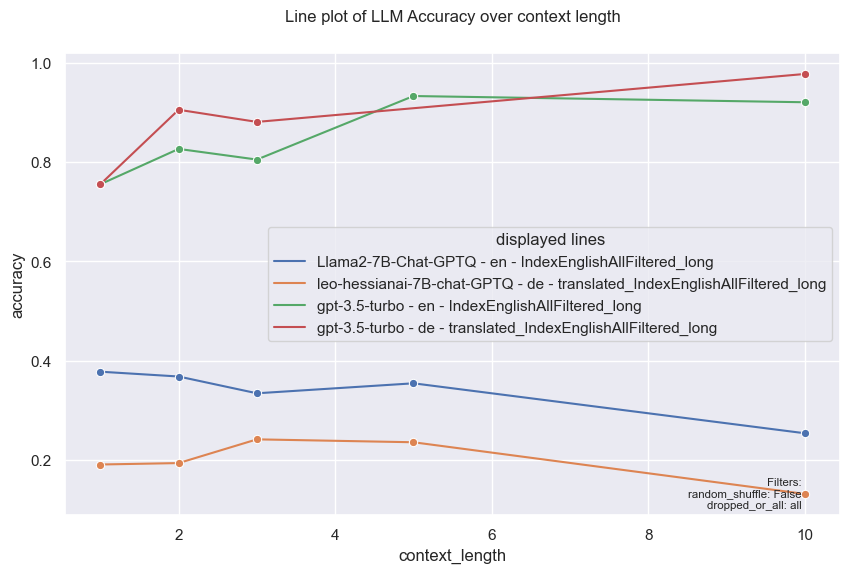
\includegraphics[width=\linewidth]{Grafiken/Evaluation/Reader/all_models_filtered_indices.png}
        \captionsetup{width=.9\linewidth}
        \caption{Comparison of all readers LLM accuracy over two indices without shuffled contexts}
        \label{fig:reader-all-overview-performance}
    \end{subfigure}%
    \begin{subfigure}{.5\textwidth}
        \centering
        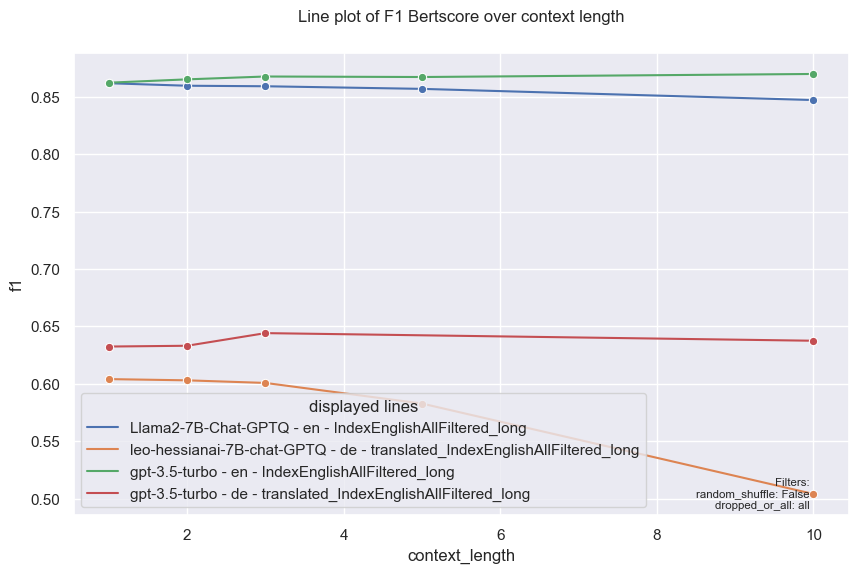
\includegraphics[width=\linewidth]{Grafiken/Evaluation/Reader/all_models_filtered_indices_f1.png}
        \captionsetup{width=.9\linewidth}
        \caption{Comparison of all readers F1 Bertscore over two indices without shuffled contexts}
        \label{fig:reader-all-overview-performance-f1}
    \end{subfigure}
    \begin{subfigure}{.5\textwidth}
        \centering
        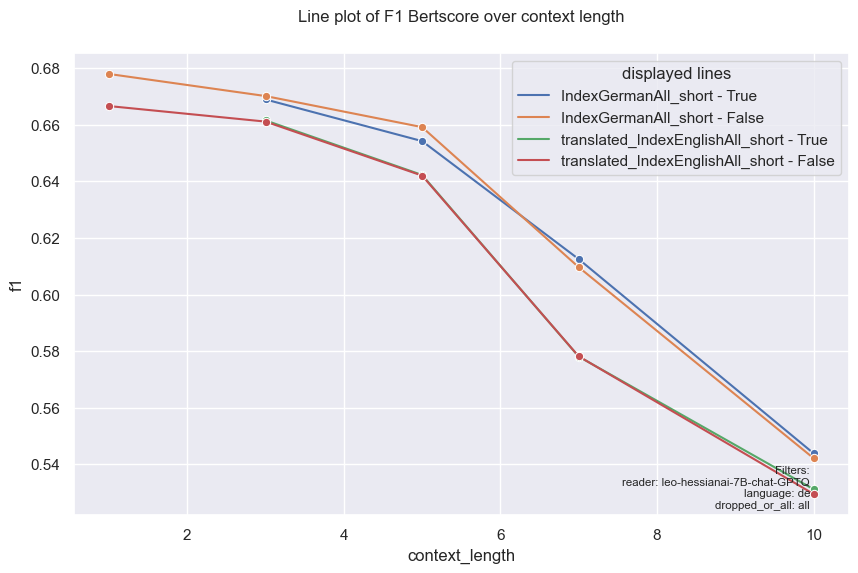
\includegraphics[width=\linewidth]{Grafiken/Evaluation/Reader/is_the_order_important_de.png}
        \captionsetup{width=.9\linewidth}
        \caption{Importance of the order of the contexts for German models}
        \label{fig:reader-importance-order-contexts-de}
    \end{subfigure}%
    \begin{subfigure}{.5\textwidth}
        \centering
        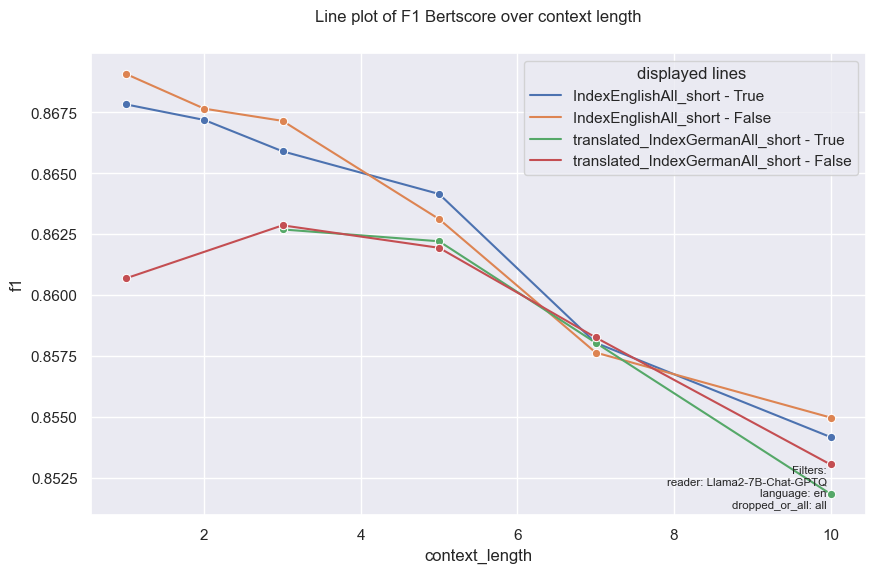
\includegraphics[width=\linewidth]{Grafiken/Evaluation/Reader/is_the_order_important_en.png}
        \captionsetup{width=.9\linewidth}
        \caption{Importance of the order of the contexts for English models}
        \label{fig:reader-importance-order-contexts-en}
    \end{subfigure}
    \caption{Multiple Reader Performance Comparisons}
    \label{fig:reader-performance}
\end{figure}

% \begin{figure}
%     \centering
%     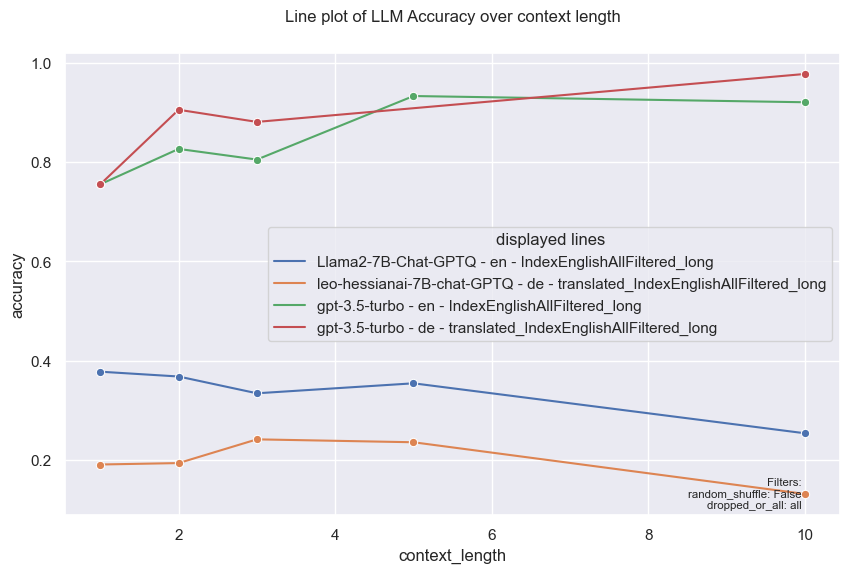
\includegraphics[width=\textwidth]{Grafiken/Evaluation/Reader/all_models_filtered_indices.png}
%     \caption{Comparison of all readers LLM accuracy over two indices without shuffled contexts}
%     \label{fig:reader-all-overview-performance}
% \end{figure}

% \begin{figure}
%     \centering
%     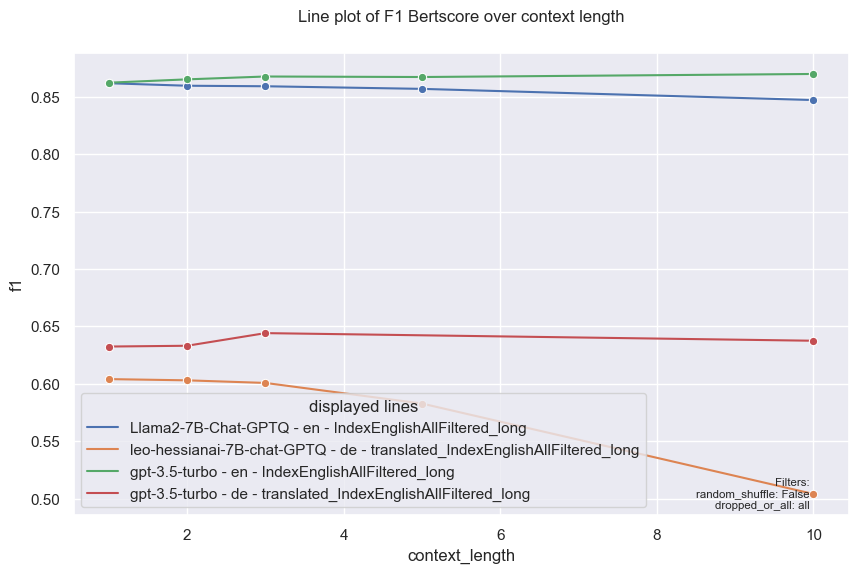
\includegraphics[width=\textwidth]{Grafiken/Evaluation/Reader/all_models_filtered_indices_f1.png} 
%     \caption{Comparison of all readers F1 Bertscore over two indices without shuffled contexts}
%     \label{fig:reader-all-overview-performance-f1}
% \end{figure}


% \begin{figure}
%     \centering
%     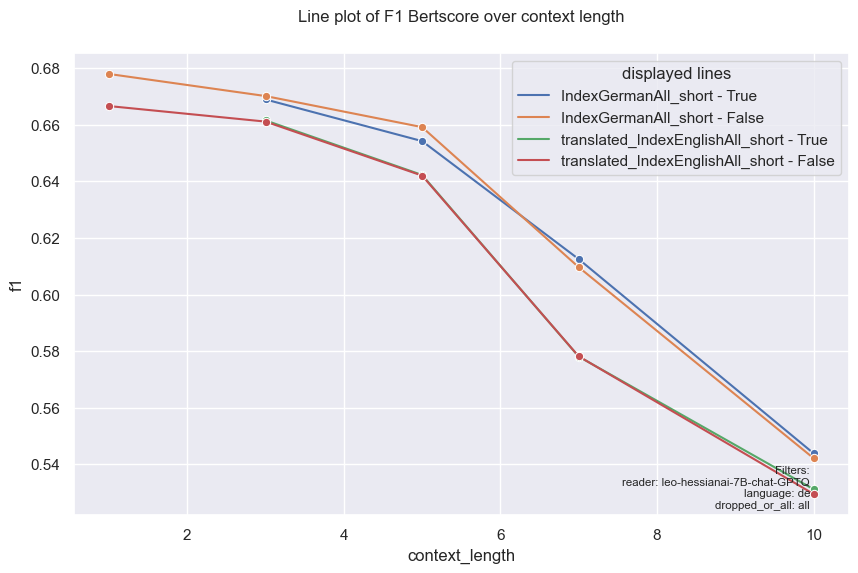
\includegraphics[width=\textwidth]{Grafiken/Evaluation/Reader/is_the_order_important_de.png} 
%     \caption{Importance of the order of the contexts for German models}
%     \label{fig:reader-importance-order-contexts-de}
% \end{figure}

% \begin{figure}
%     \centering
%     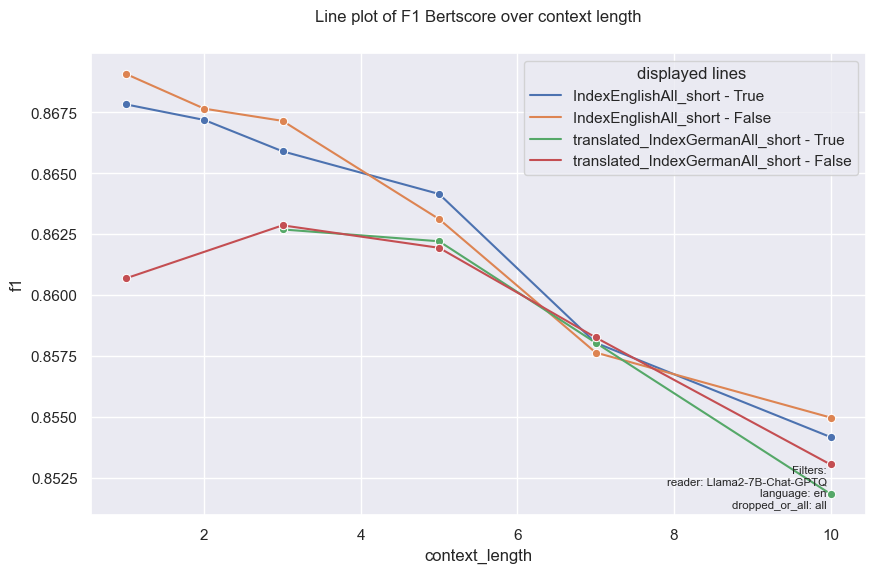
\includegraphics[width=\textwidth]{Grafiken/Evaluation/Reader/is_the_order_important_en.png} 
%     \caption{Importance of the order of the contexts for English models}
%     \label{fig:reader-importance-order-contexts-en}
% \end{figure}

% \begin{figure}
%     \centering
%     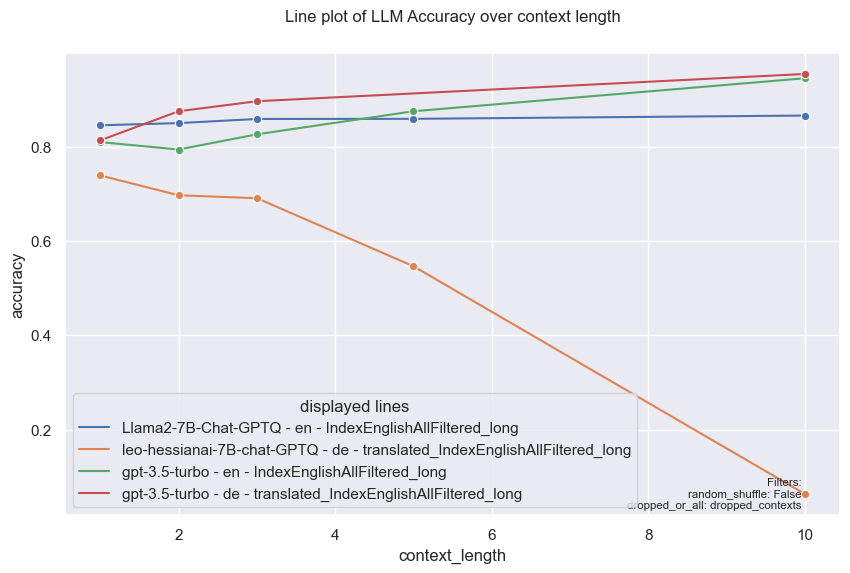
\includegraphics[width=.8\textwidth]{Grafiken/Evaluation/Reader/context_dropped.png} 
%     \caption{Comparison of the influence of context dropping on the performance of the readers}
%     \label{fig:reader-context-drop}
% \end{figure}


% \begin{figure}
%     \centering
%     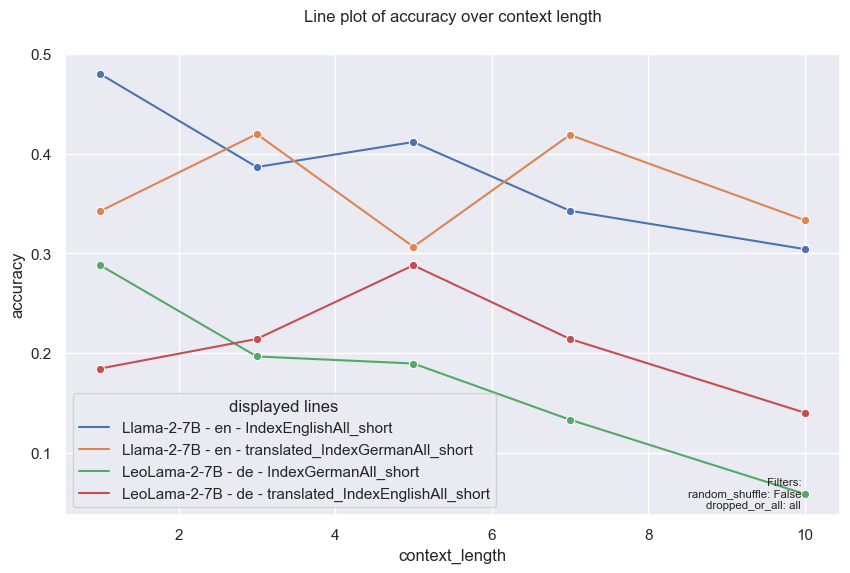
\includegraphics[width=\textwidth]{Grafiken/Evaluation/Reader/all_indices_all_readers_no_shuffle.png}
%     \caption{Comparison of all Readers over all Indices without shuffled contexts}
%     \label{fig:reader-all-overview-performance}
% \end{figure}
\subsection{Conversational Question Answering Results}
\label{subsec:convqa-results}
